% a simple template with cesbio color code

\documentclass[xcolor=table, t, aspectratio=169]{beamer} 
\graphicspath{{../FIGURES/}}
\usepackage[utf8]{inputenc}
\usepackage{booktabs, comment} 
\usepackage[absolute, overlay]{textpos} 
\usepackage{pgfpages}
\usepackage{caption}
\usepackage[font=footnotesize]{caption}
\usepackage{multirow}
\usepackage{hyperref}
\usepackage{blindtext}
\usepackage{amsmath}
\usepackage[makeroom]{cancel}
\usepackage{textpos}
\usepackage{tikz}
\usepackage{csquotes}
\usepackage{graphicx}


% CESBIO ADAPTED COLOURS 
\definecolor{colorLAERO}{RGB}{67, 141, 204}
\definecolor{forestgreen}{rgb}{0.13, 0.55, 0.13}
\definecolor{greenyellow}{rgb}{0.68, 1.0, 0.18}
\definecolor{inchworm}{rgb}{0.7, 0.93, 0.36}

% OPTIONAL COLOURS
% you can add the ones you need : lot of proposition on http://latexcolor.com/
\definecolor{ballblue}{rgb}{0.13, 0.67, 0.8}
\definecolor{bluegreen}{rgb}{0.0, 0.87, 0.87}
\definecolor{chromeyellow}{rgb}{1.0, 0.65, 0.0}
\definecolor{darkcyan}{rgb}{0.0, 0.55, 0.55}
\definecolor{darkpastelred}{rgb}{0.76, 0.23, 0.13}
\definecolor{electricgreen}{rgb}{0.0, 1.0, 0.0}
\definecolor{electriclime}{rgb}{0.8, 1.0, 0.0}
\definecolor{deepcarrotorange}{rgb}{0.91, 0.41, 0.17}
\definecolor{ganttblue}   {HTML}{2B6CB0}
\definecolor{ganttcyan}   {HTML}{2C7A7B}
\definecolor{ganttgreen}  {HTML}{276749}
\definecolor{ganttorange} {HTML}{C05621}
\definecolor{ganttgray}   {HTML}{4A5568}
\definecolor{ganttbg}     {HTML}{EBF4FF}
\definecolor{ganttbar}    {HTML}{BEE3F8}
\definecolor{milestonecol}{HTML}{E53E3E}


% CESBIO ADAPTED BEAMER OPTIONS
\setbeamercolor{title in head/foot}{bg=inchworm, fg=forestgreen}
\setbeamercolor{author in head/foot}{bg=colorLAERO}
\setbeamertemplate{page number in head/foot}{}

\useoutertheme{infolines}
\usetheme{Warsaw}
\usecolortheme[named=colorLAERO]{structure}


% SPECIFIC COMMANDS
% if you nee to set command for youe presentation, you can put them here
\newcommand{\defnotation}[1]{\bf{\textsl{#1}}}

\usepackage[
citestyle=abbrv, 
bibstyle=abbrv,
style=authoryear, %-comp,
backend=biber
%maxbibnames=99, % Make sure we are printing all authors in the appendix
]{biblatex}

\usepackage{pgfgantt}
\usepackage{helvet}
% PRESENTATION INFORMATIONS
% to fill in

% \title[]{}
% \subtitle{Subtitle}

\usetikzlibrary{positioning, calc}
\usetikzlibrary{calc}

% ── Colours (adapt to your theme) ─────────────────────────────────────────────
\definecolor{titleblue}  {HTML}{1A365D}
\definecolor{accentblue} {HTML}{2B6CB0}
\definecolor{lightgray}  {HTML}{EDF2F7}
\definecolor{medgray}    {HTML}{718096}

% ── Metadata ──────────────────────────────────────────────────────────────────
\author[J.~Hedman]{Johan Hedman}
\institute[LAERO]{Laboratoire d'Aérologie (LAERO) · Université de Toulouse}
\date{\today}

% ── Title frame ───────────────────────────────────────────────────────────────
% Use a fully custom frame instead of \titlepage for full layout control
\newcommand{\customtitleframe}{%
\begin{frame}[plain]
	\begin{tikzpicture}[remember picture, overlay]
		
		%% ── Background ─────────────────────────────────────────────────────────────
		\fill[titleblue]
		(current page.north west) rectangle
		($(current page.north east) + (0, -0.38\paperheight)$);
		
		\fill[accentblue]
		($(current page.north west) + (0, -0.38\paperheight)$) rectangle
		($(current page.north east) + (0, -0.405\paperheight)$);
		
		%% ── Title block ────────────────────────────────────────────────────────────
		\node[anchor=west, text=white, font=\large\bfseries, text width=0.95\paperwidth,] at 
		($(current page.north west) + (0.7cm, -0.13\paperheight)$)
		{Etude des rouleaux de couche limite sous les tempêtes};
		
		\node[anchor=west, text=white!70!titleblue, font=\small,text width=0.85\paperwidth,] at 
		($(current page.north west) + (0.7cm, -0.26\paperheight)$)
		{Johan Hedman \quad·\quad LAERO, Université de Toulouse \quad·\quad \insertdate};
		
		%% ── Supervisors ────────────────────────────────────────────────────────────
		\node[anchor=north west, font=\bfseries\small\color{accentblue}] at 
		($(current page.north west) + (0.7cm, -0.405\paperheight - 0.52cm)$)
		{Supervision};
		
		\node[anchor=north west, font=\footnotesize\color{titleblue}, align=left, text width=0.38\paperwidth]
		at ($(current page.north west) + (0.7cm, -0.405\paperheight - 1.0cm)$)
		{%
			\textbf{Prof. Jean-Pierre Chaboureau} \\
			\textcolor{medgray}{LAERO, Université de Toulouse} \\[5pt]
		};
		
		%% ── Divider ────────────────────────────────────────────────────────────────
		\draw[accentblue!30, line width=0.5pt]
		($(current page.north west) + (0.50\paperwidth, -0.405\paperheight - 0.50cm)$) --
		($(current page.south west) + (0.50\paperwidth, 0.45cm)$);
		
		%% ── Jury ───────────────────────────────────────────────────────────────────
		\node[anchor=north west, font=\bfseries\small\color{accentblue}]at ($(current page.north west) + (0.53\paperwidth, -0.405\paperheight - 0.52cm)$)
		{Membre du CSI};
		
		\node[anchor=north west, font=\footnotesize\color{titleblue}, align=left, text width=0.42\paperwidth]
		at ($(current page.north west) + (0.53\paperwidth, -0.405\paperheight - 1.0cm)$)
		{%
			\textbf{Prof } \textcolor{medgray}{\textit{}} \\
			\textbf{Prof.~Firstname Lastname} \textcolor{medgray}{\textit{}} \\
		};
		
		%% ── Logo strip ─────────────────────────────────────────────────────────────
		\fill[white]
		($(current page.south west) + (0, 0.10\paperheight)$)
		rectangle (current page.south east);
		
		\draw[accentblue!25, line width=0.4pt]
		($(current page.south west) + (0, 0.10\paperheight)$) --
		($(current page.south east) + (0, 0.10\paperheight)$);
		
		\node[anchor=south west, xshift=0.5cm, yshift=0.20cm] at (current page.south west)		{
\includegraphics[height=1.5cm]{LOGO/LAERO-logo.jpg}};
		
		\node[anchor=south, yshift=0.25cm] at (current page.south)
			{
\includegraphics[height=1.0cm]{LOGO/UNIV-logo.png}\hspace{1cm}%
			
\includegraphics[height=1.20cm]{LOGO/CNRS-logo.jpeg}};
		
		\node[anchor=south east, xshift=-0.5cm, yshift=0.20cm] at (current page.south east)
		{
\includegraphics[height=1.2cm]{LOGO/logo-IRD.png}};
		
	\end{tikzpicture}
\end{frame}
}





% cesbio adapted frame structure
\addtobeamertemplate{navigation symbols}{}{%
    \usebeamerfont{footline}%
    \usebeamercolor[fg]{footline}%
    \hspace{1em}%
    \insertframenumber/\inserttotalframenumber
}

\usepackage{soul}
\makeatletter
\let\HL\hl
\renewcommand\hl{%
  \let\set@color\beamerorig@set@color
  \let\reset@color\beamerorig@reset@color
  \HL}
\makeatother

\addbibresource{../../groupeThese.bib}
\graphicspath{{FIGURES/}}

%Title Page
\title{Réunion Mercredi 29/04/2026}
\author{}

\usepackage[caption = false]{subfig}
\begin{document}
\begin{frame}
\maketitle
\end{frame}

\begin{frame}{Dernière discussion}
Ce qu'on avait dit
  \begin{itemize}
    \item Problématique de diagnostique de BLH pouvait expliquer les rouleaux trop peu espacés dans le cas ADRIAN
  \end{itemize}
\end{frame}


\begin{frame}{Cadre de la tempête Alex}
\begin{minipage}{0.3\textwidth}
	\centering
	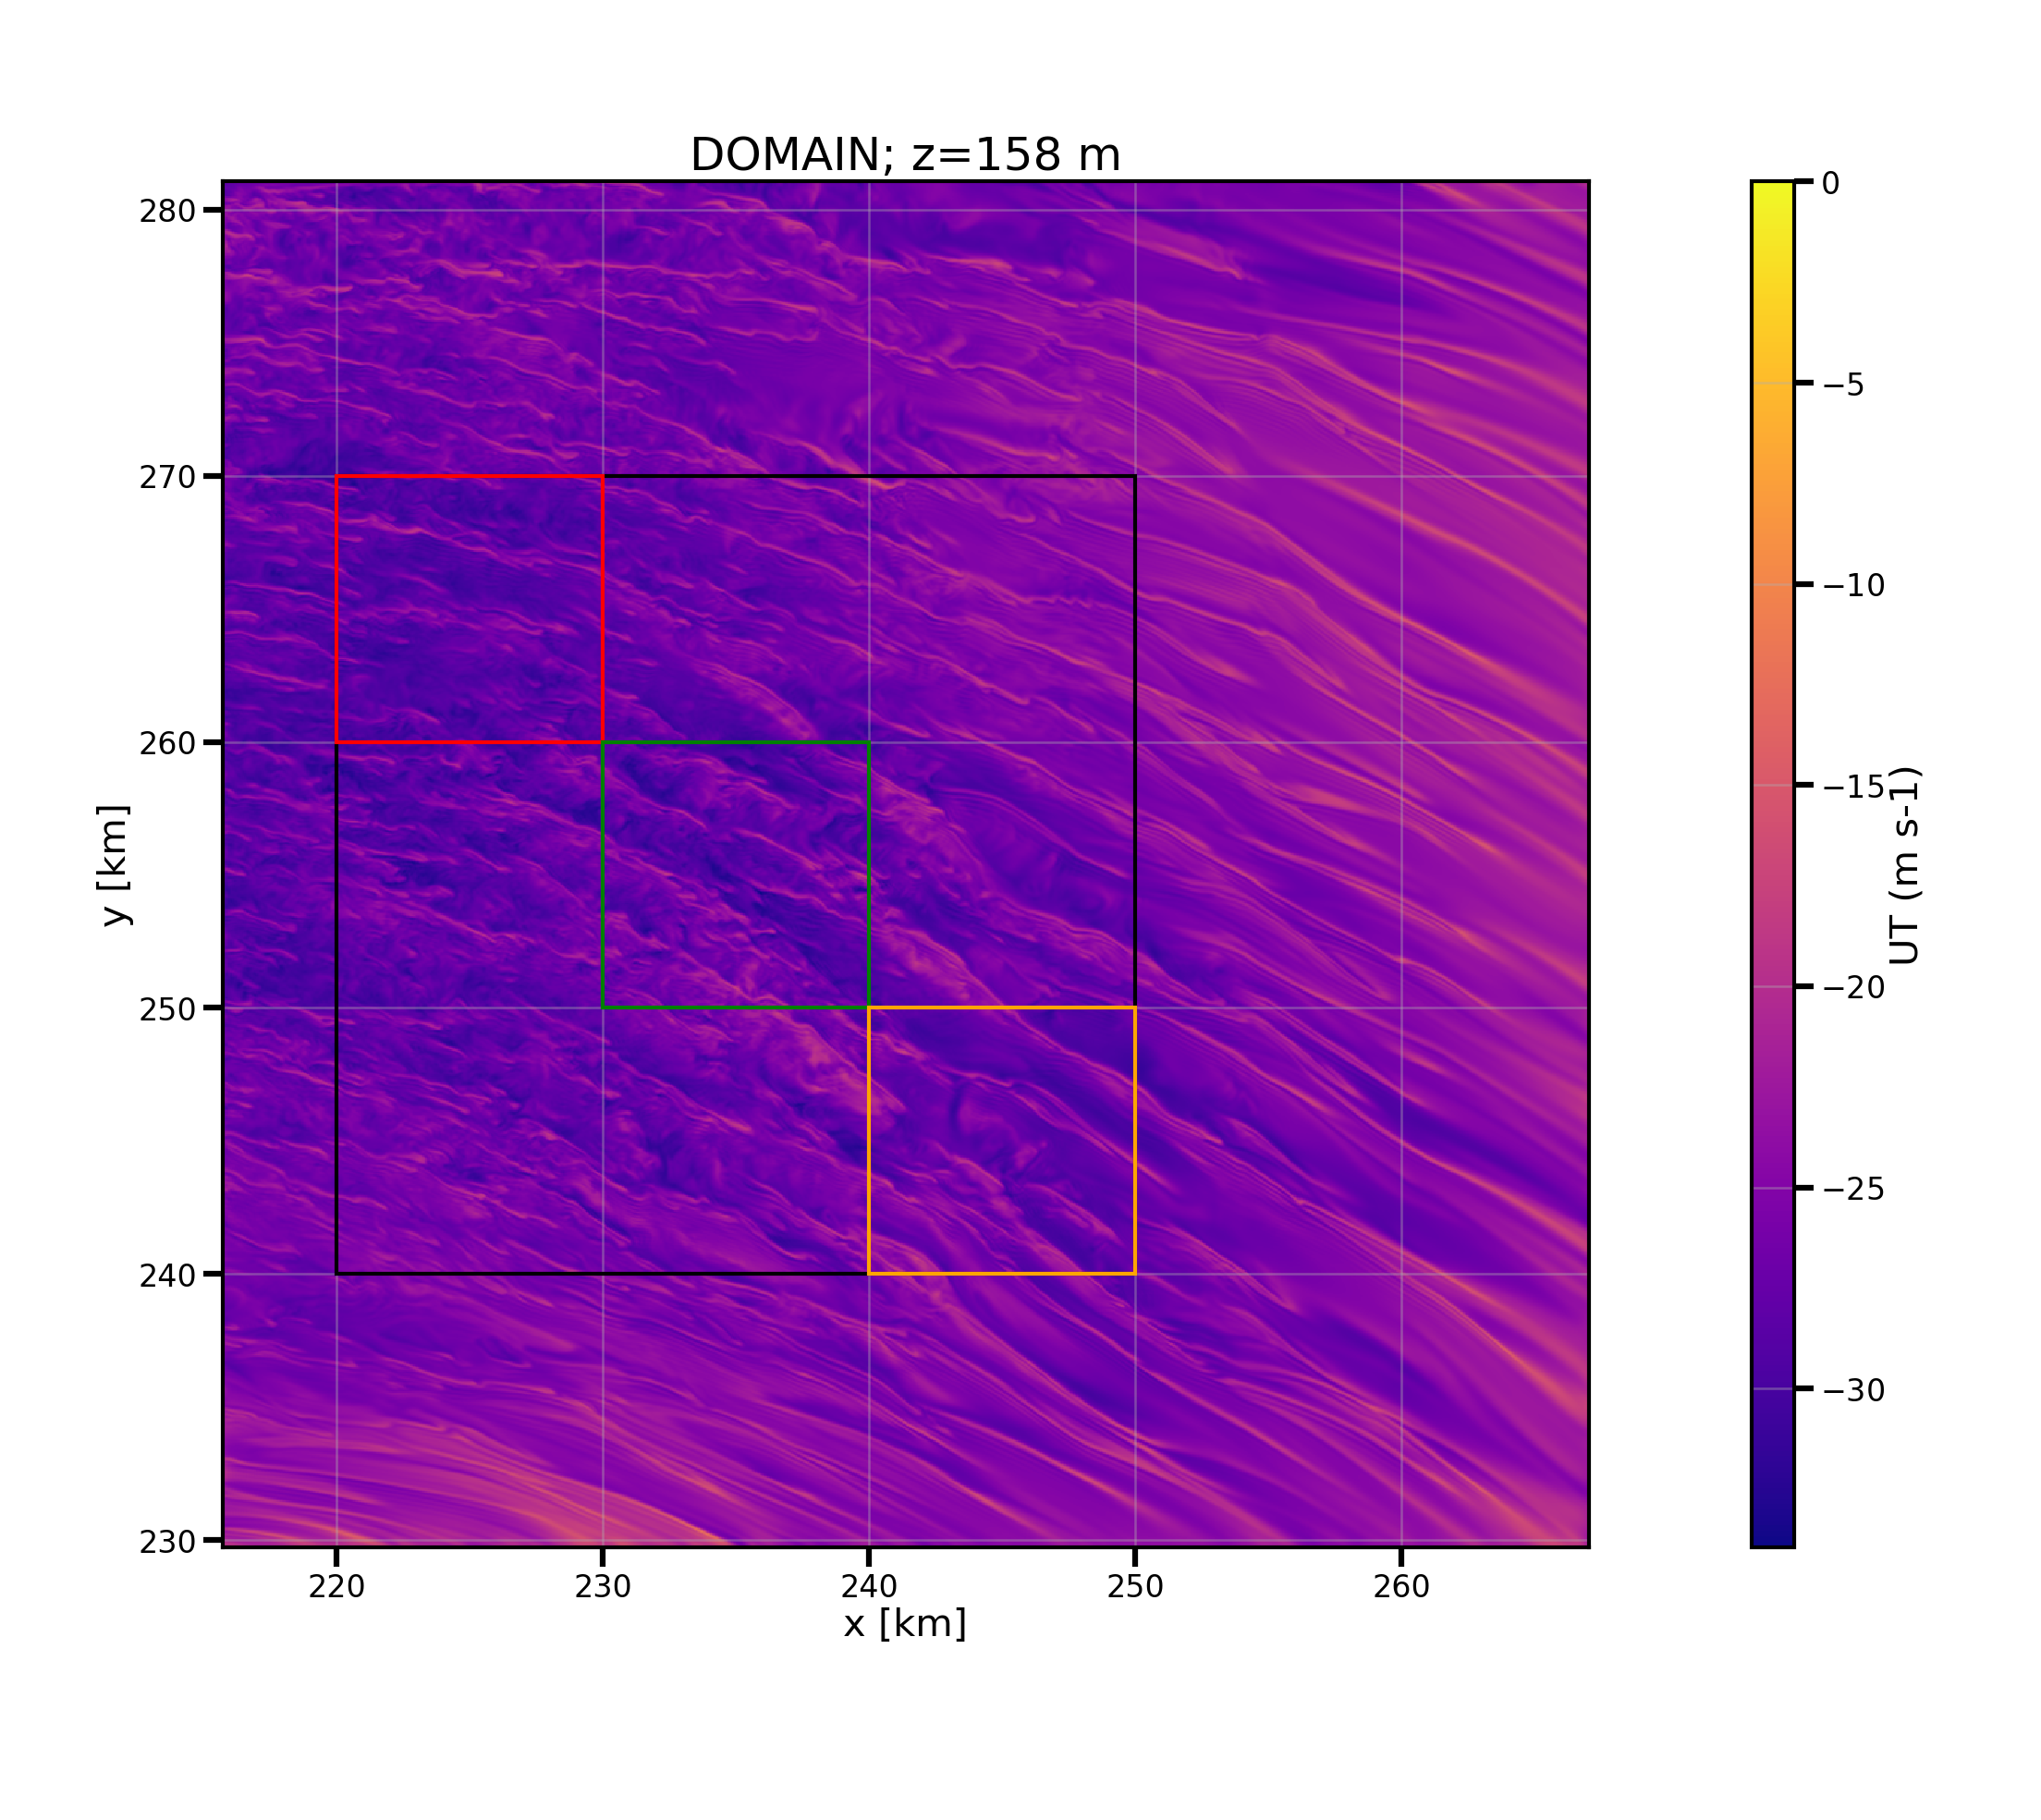
\includegraphics[width=\linewidth]{DOMAIN/WHOLEDOMAIN.png}
\end{minipage}
\hfill
\begin{minipage}{0.65\textwidth} 
  \centering
  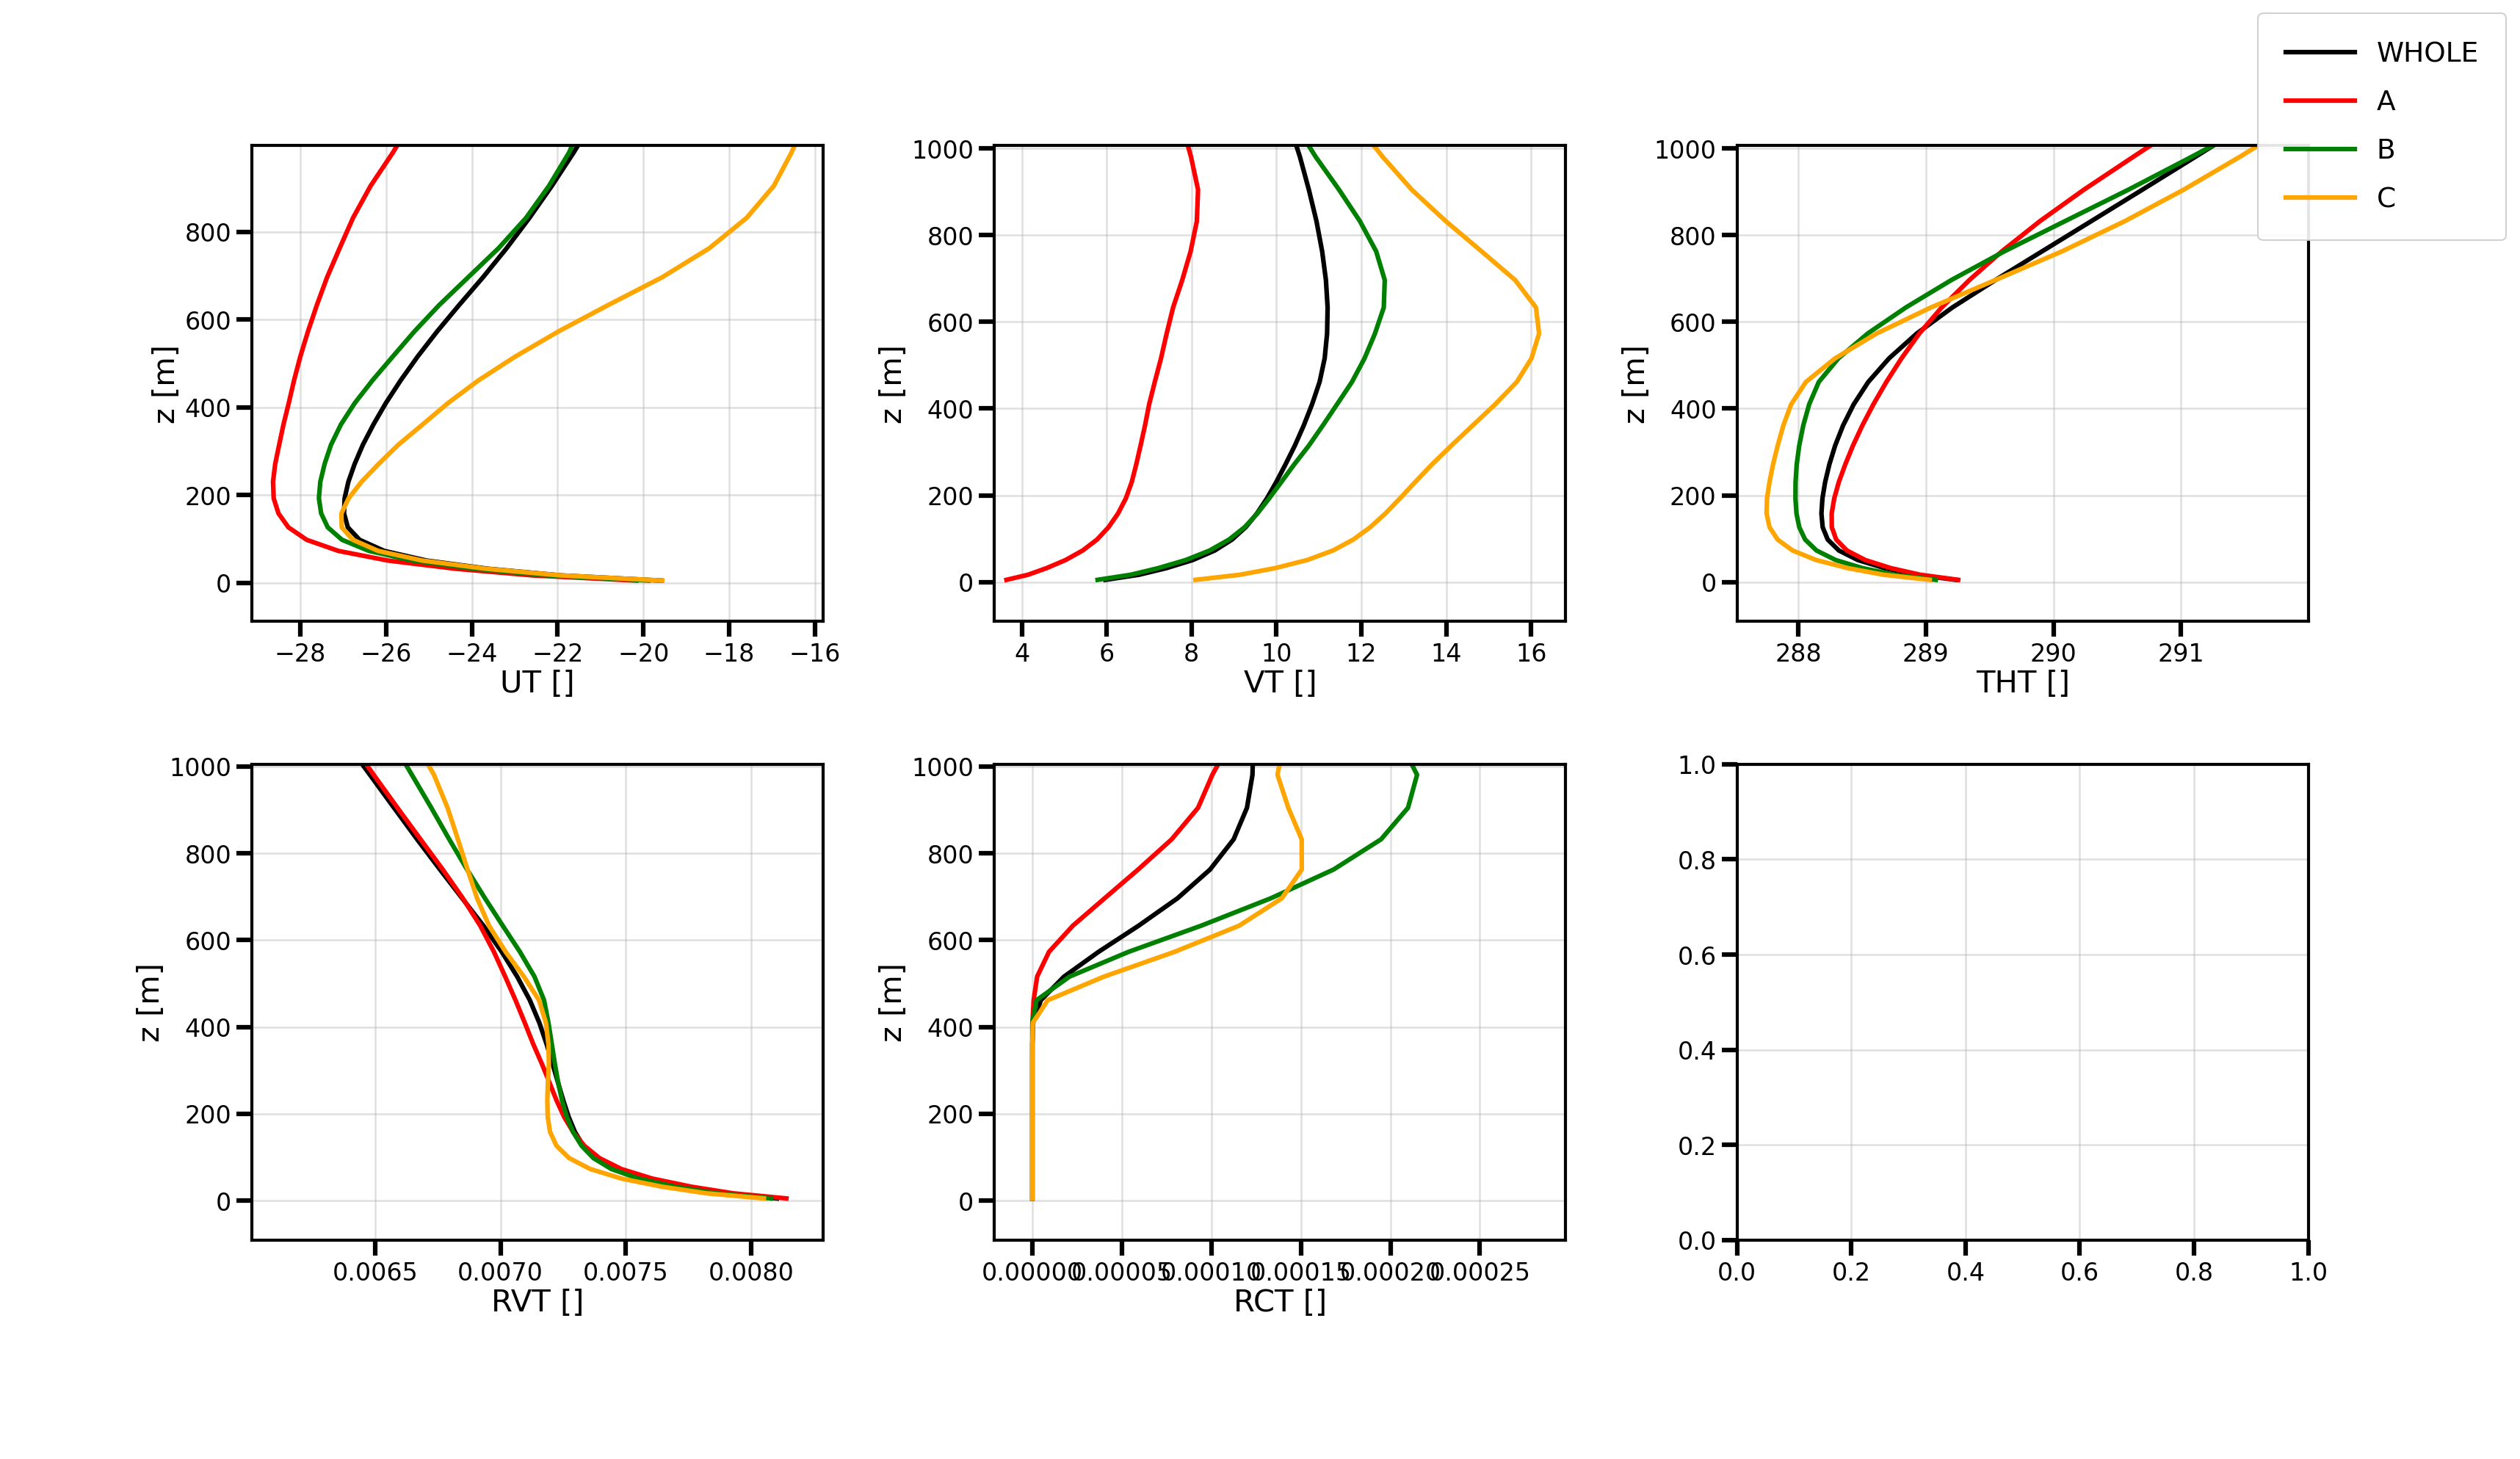
\includegraphics[width=\linewidth]{DOMAIN/rectprofiles.png}
\end{minipage}
Simulations LES à partir des profils moyens de : UT, VT, THT, RVT \\
Les profils de UT, VT, RVT sont rappelés avec une constante de rappel $\tau = 60s$. 
\end{frame}

\begin{frame}{Zoom sur les profils de vents dans le domaine de référence}
Recherche des points d'inflexion sur l'écoulement moyen perpendiculaire aux rouleaux, i.e. approx v (Weckwerth et al, 1996)
	\begin{minipage}{0.8\textwidth}
		\centering
		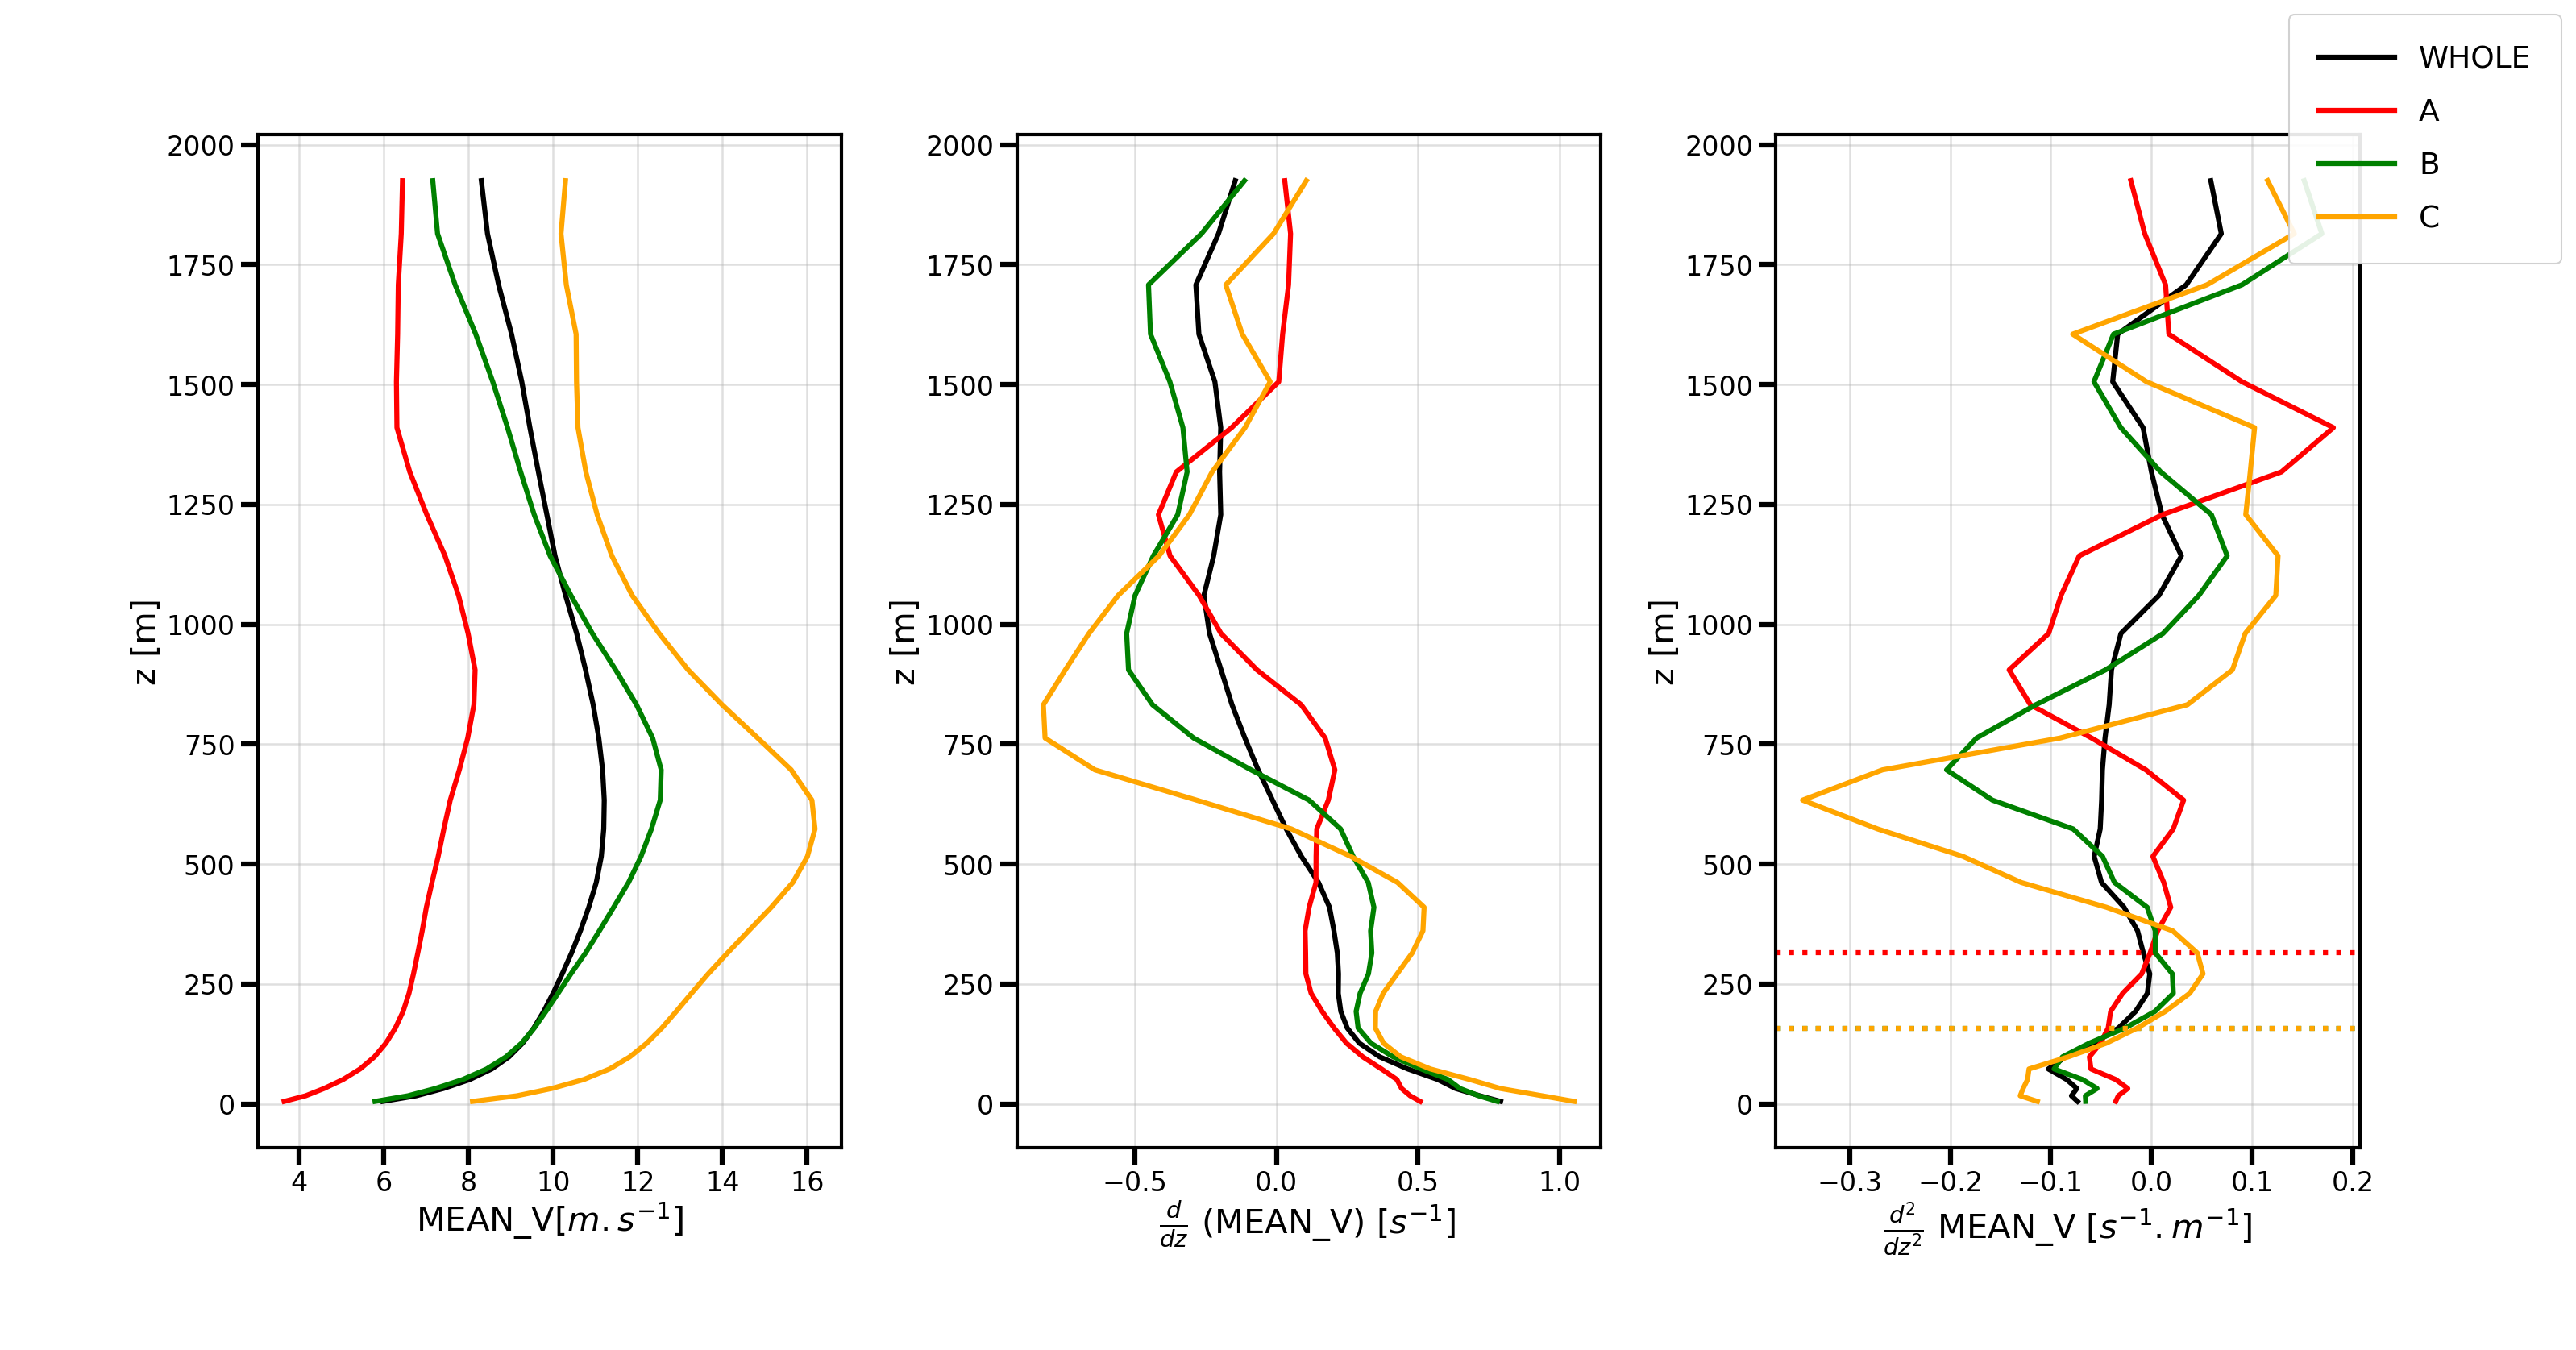
\includegraphics[width=\linewidth]{DOMAIN/analyse_wind.png}
	\end{minipage}
\end{frame}

\begin{frame}{Comparaison dans domaine A}
	\begin{minipage}{0.65\textwidth}
		\centering
		
\includegraphics[width=\linewidth]{domA/comp_cut.png}
		Dx(LES = 25m) !!\\
				\begin{tabular}{c|cc}
			&  LHF   & SHF \\
			\hline
			LES  & 363.81 &  \hl{42.09 }\\
			ALEX & 394.27 & 220.64 \\
		\end{tabular}
	\end{minipage}
	\hfill
		\begin{minipage}{0.34\textwidth}
		\centering
		
\includegraphics[width=0.9\linewidth]{LESdomA/spectr.png}
		
\includegraphics[width=0.9\linewidth]{LESdomA/evol.png}
	\end{minipage}
\end{frame}

\begin{frame}{Comparaison dans domaine C}
	\begin{minipage}{0.65\textwidth}
		\centering
		
\includegraphics[width=0.8\linewidth]{domC/comp_cut.png}
		\begin{tabular}{c|cc}
			&  LHF   & SHF \\
			\hline
			LES  & 412.78 &  \hl{66.0}  \\
			ALEX & 451.15 & 280.33 \\
		\end{tabular} \\
		\vspace{0.2cm}
		Paramétrisation flux ECUME6 vs ECUME ?
	\end{minipage}
	\hfill
	\begin{minipage}{0.34\textwidth}
			\centering
			
\includegraphics[width=0.9\linewidth]{LESdomC/spectr.png}
			
\includegraphics[width=0.9\linewidth]{LESdomC/evol.png}
	\end{minipage}
\end{frame}

\begin{frame}{Discussion}
	\begin{itemize}
		\item SHF: problème ! \\
		peut être paramétrisation ECUME - ECUME6 ? \\
		Ou $\Delta \theta$ incorrect 
		\item Spectre maoyenné sur altitude
	\end{itemize}
\end{frame}


% =======================================================================================
% =======================================================================================
\section{SHF fluxes}
\begin{frame}
\sectionpage
\vfill 
Différence majeure entre LES idéalisée et ALEX cas réel = les flux de chaleur sensibles. \\
\vfill
Différentes pistes à explorer pour expliquer ces différences dans le cadre d'un flux paramétré par param bulk (\cite{lfarhImpactSurfaceTurbulent2024}).
$$H_{bulk} = \rho c_p C_H U \Delta \theta $$ \\
\end{frame}

\subsection{Problème dans les flux}


\subsection{Piste1: Choix de paramétrisation}
\begin{frame}{Deux param différentes: ECUME et ECUME6}
	ECUME (rouge) et ECUME6 (violet) sont des parazmétrisations issues de campagnes en mer. ECUME seulement avec des vents modérés et faibles. \\
	\begin{minipage}{1\textwidth}
		\centering
		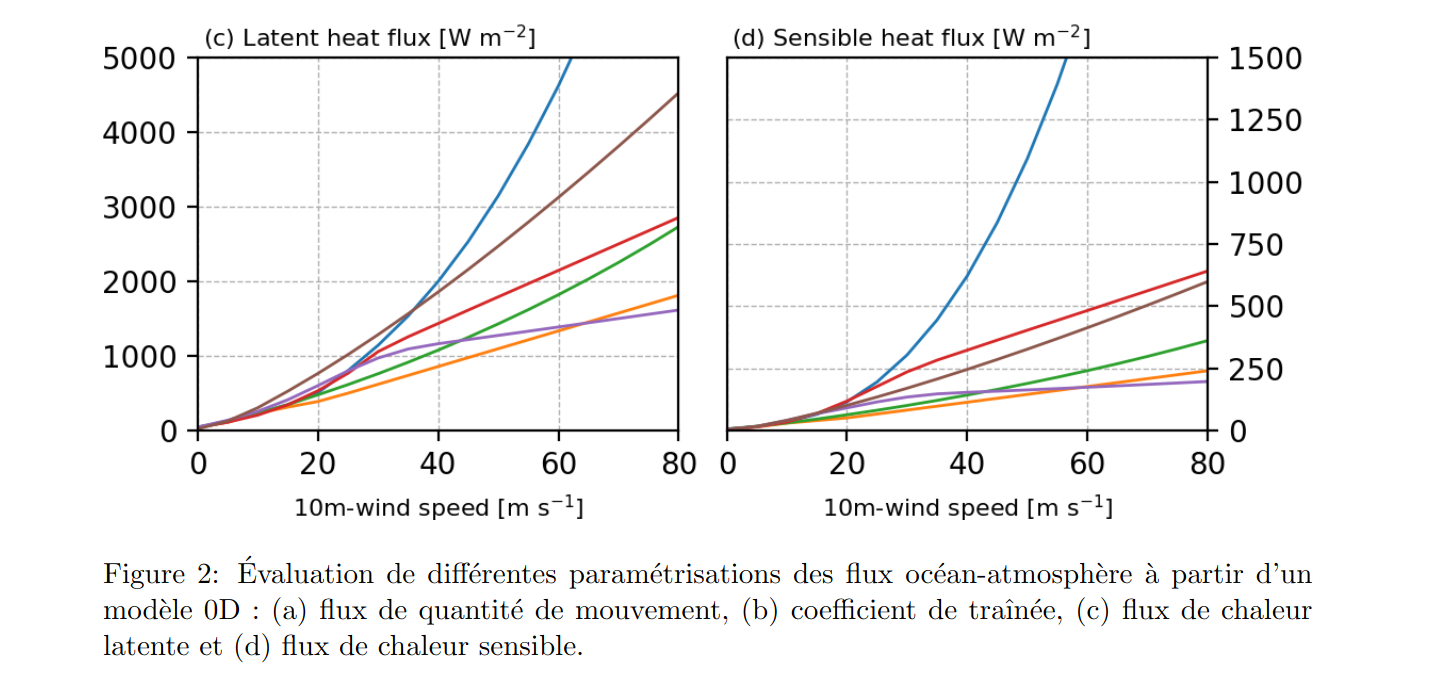
\includegraphics[width=0.7\linewidth]{FIGURES/ECUME.png}
	\end{minipage}
	\\
	Différence des flux mais pas du même ordre de grandeurs !  
\end{frame}

\begin{frame}{Domaine C avec ECUME6 et ECUME}
	\begin{minipage}{0.48\textwidth}
		\centering
		
\includegraphics[width=1\linewidth]{domC/comp_cut.png}
		\begin{tabular}{c|cc}
			&  LHF   & SHF \\
			\hline
			LES  & 412.78 &  \hl{66.0}  \\
			ALEX & 451.15 & 280.33 \\
		\end{tabular} \\
		\vspace{0.5cm}
		ECUME6 dans la LES
	\end{minipage}
	\hfill
	\begin{minipage}{0.48\textwidth}
		\centering
		
\includegraphics[width=1\linewidth]{domC_ECUME/comp_cut.png}
		\begin{tabular}{c|cc}
			&  LHF   & SHF \\
			\hline
			LES  & 384.86 &  \hl{95.67}  \\
			ALEX & 451.15 & 280.33 \\
		\end{tabular} \\
		\vspace{0.5cm}
		ECUME dans la LES
	\end{minipage}
\end{frame}



\subsection{Piste2: Résolution verticale}
\begin{frame}{Différence de résolution verticale}
	\begin{minipage}{0.48\textwidth}
	\centering
	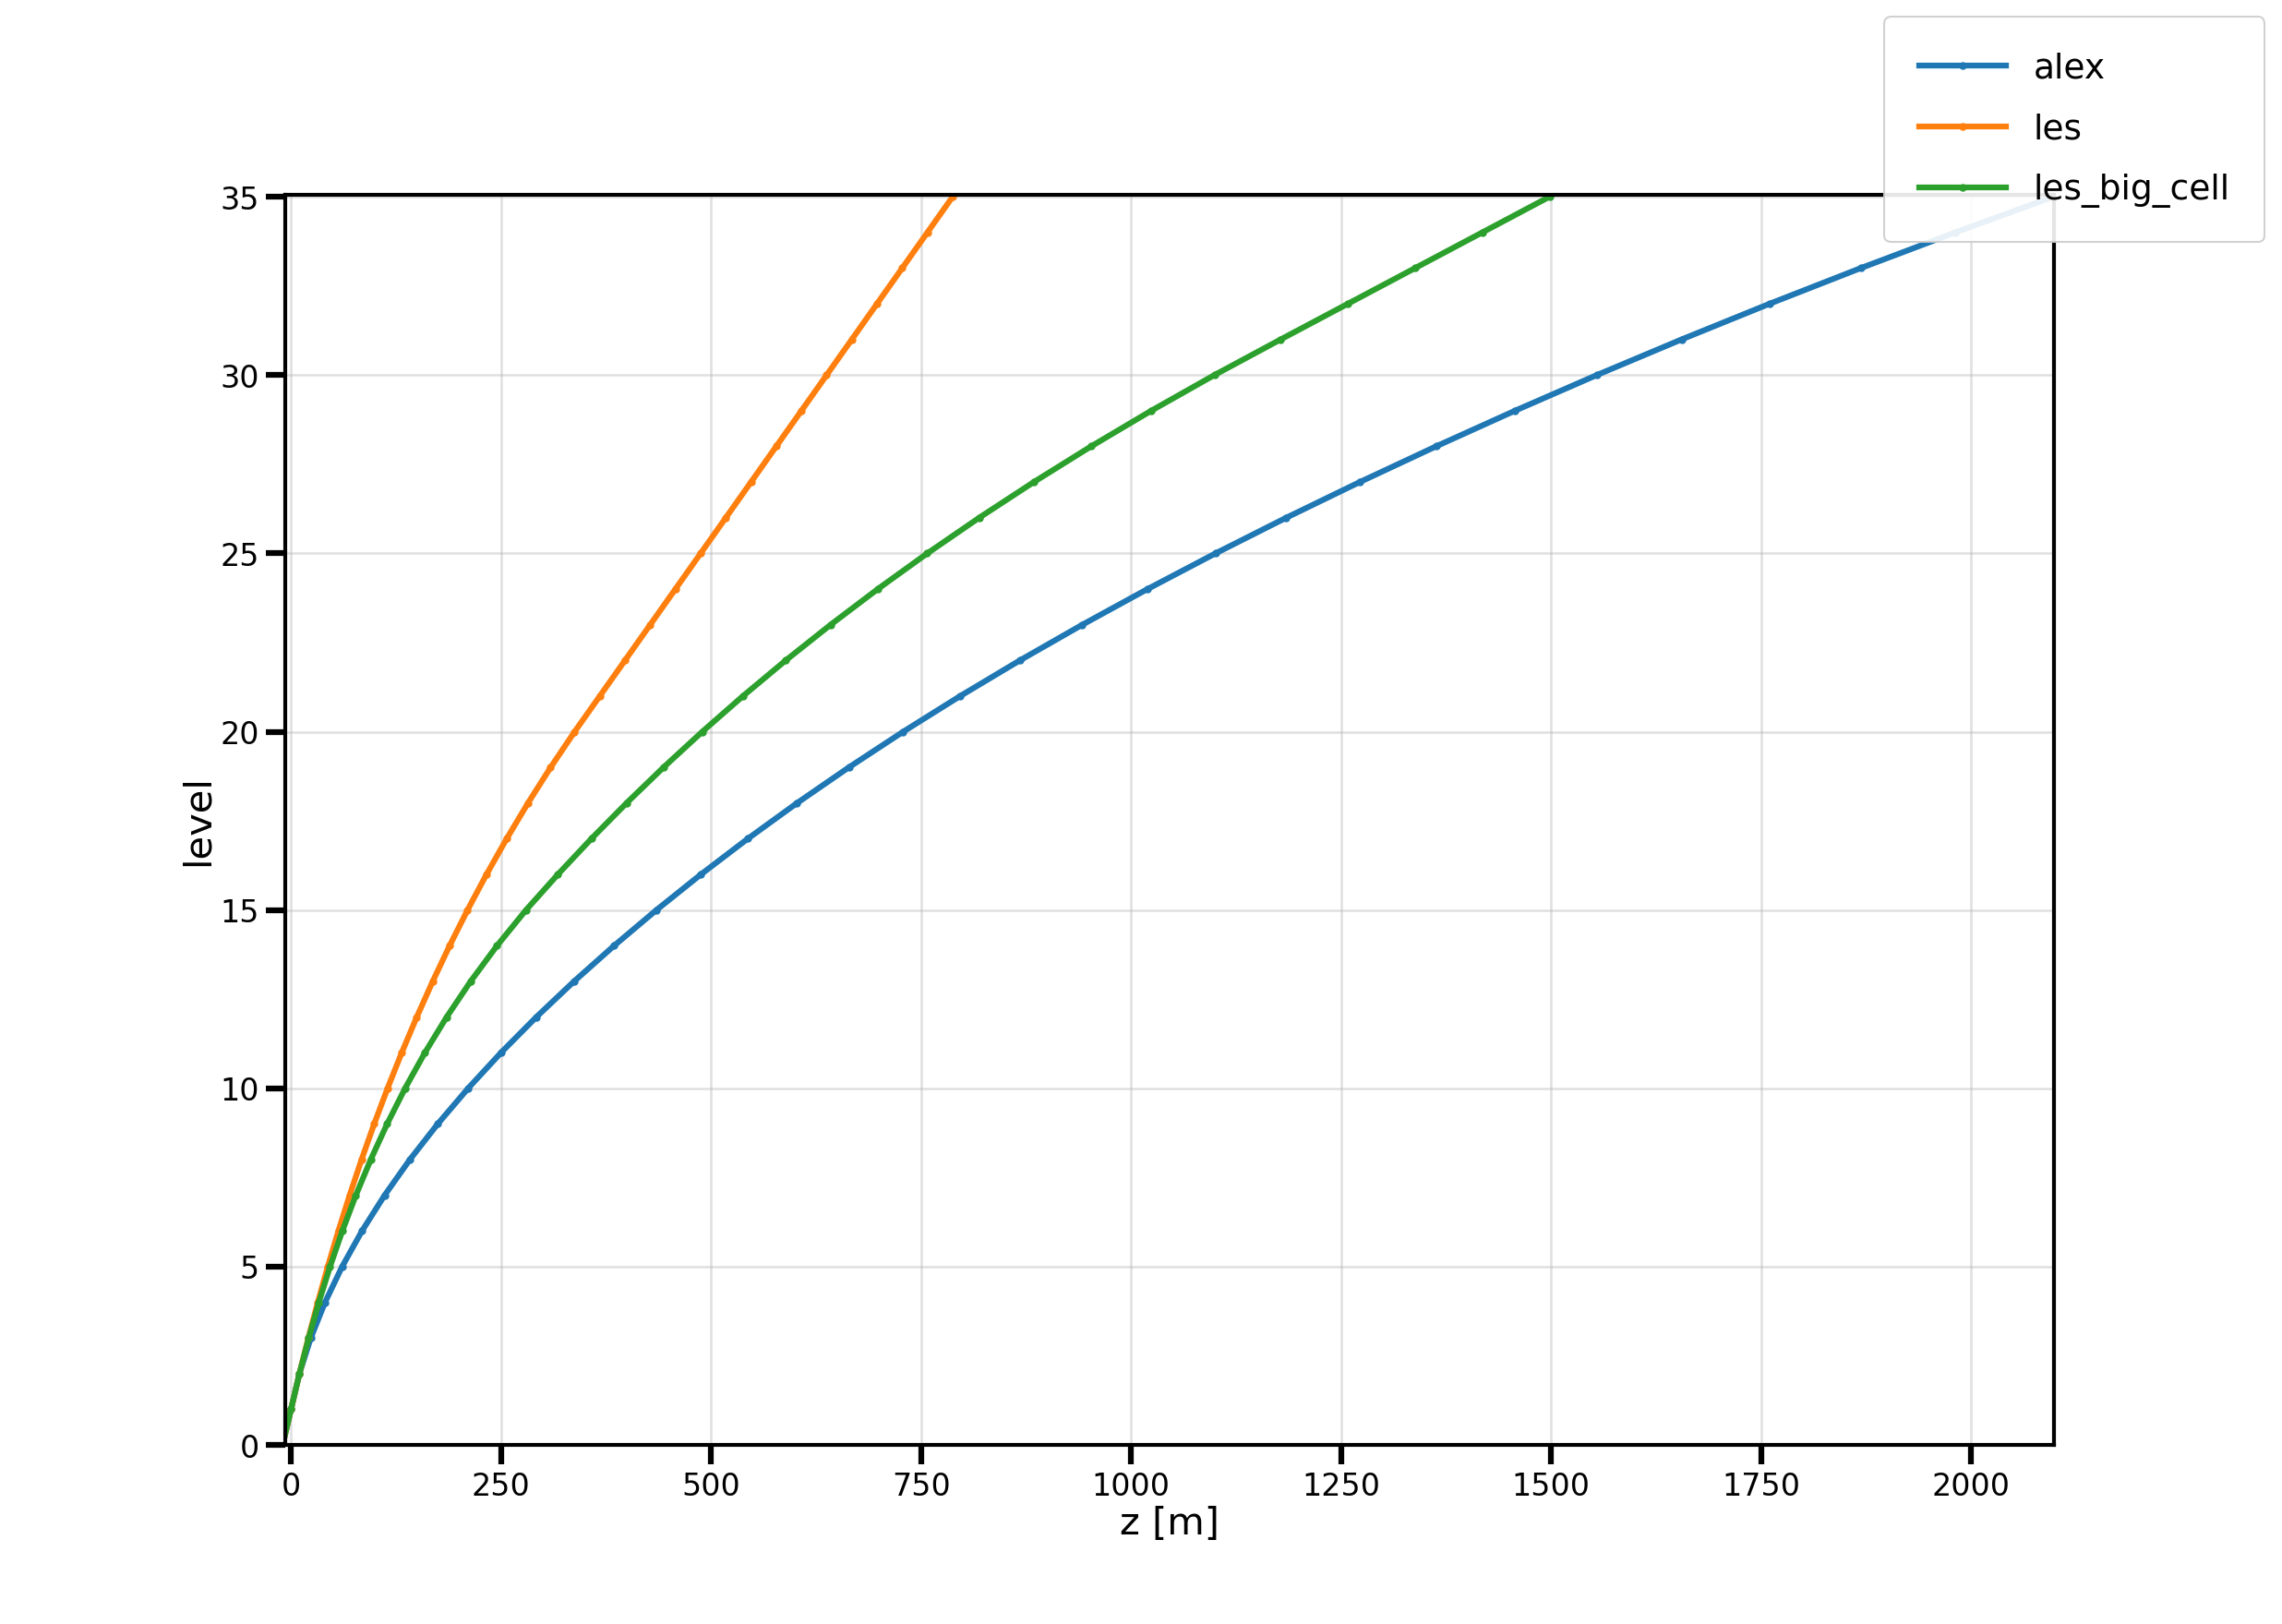
\includegraphics[width=1\linewidth]{LESdomC/grille.png}
\end{minipage}
	\hfill
\begin{minipage}{0.48\textwidth}
	\centering
	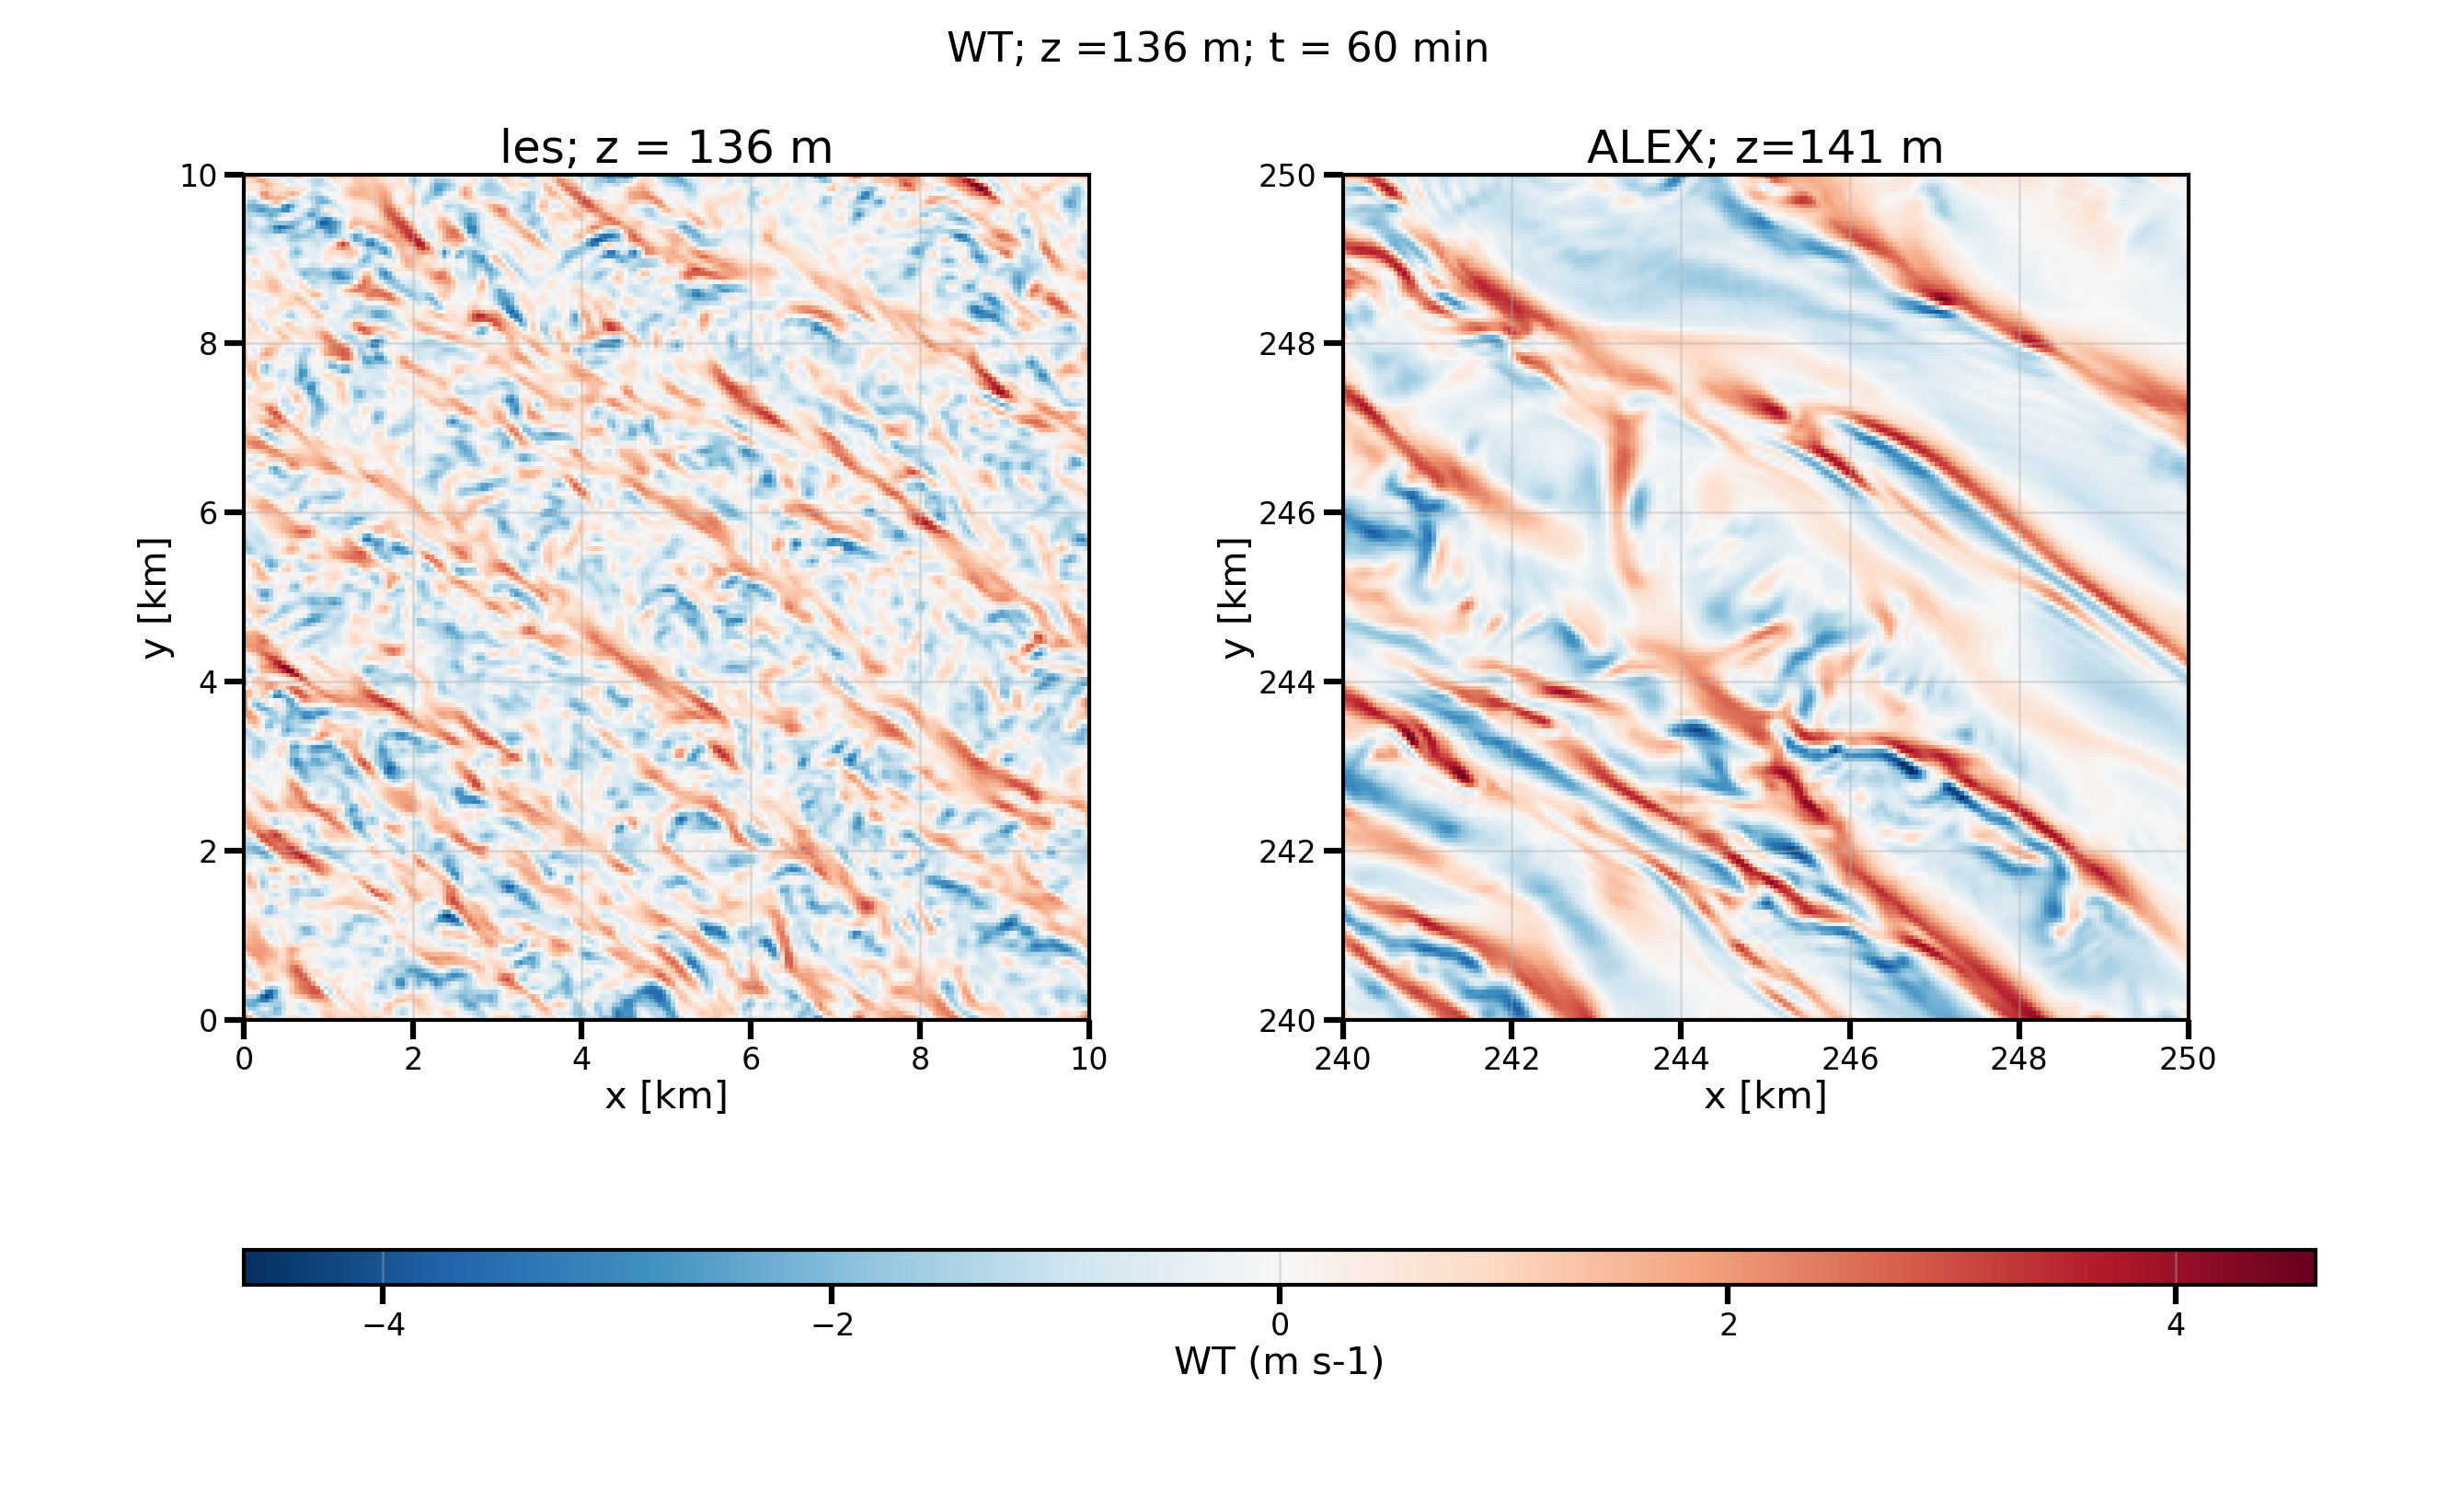
\includegraphics[width=1\linewidth]{bigLESdomC/comp_cut.png}
	\begin{tabular}{c|cc}
		&  LHF   & SHF \\
		\hline
		LES  & 401.13 &  68.16  \\
		ALEX & 451.15 & 280.33 \\
	\end{tabular} \\
	\vspace{0.5cm}
\end{minipage}
\end{frame}

\subsection{Piste3: Différence de température de la première couche atmosphérique}
\begin{frame}{Différence de température de la première couche atmosphérique}
	\begin{minipage}{0.48\textwidth}
		\centering
		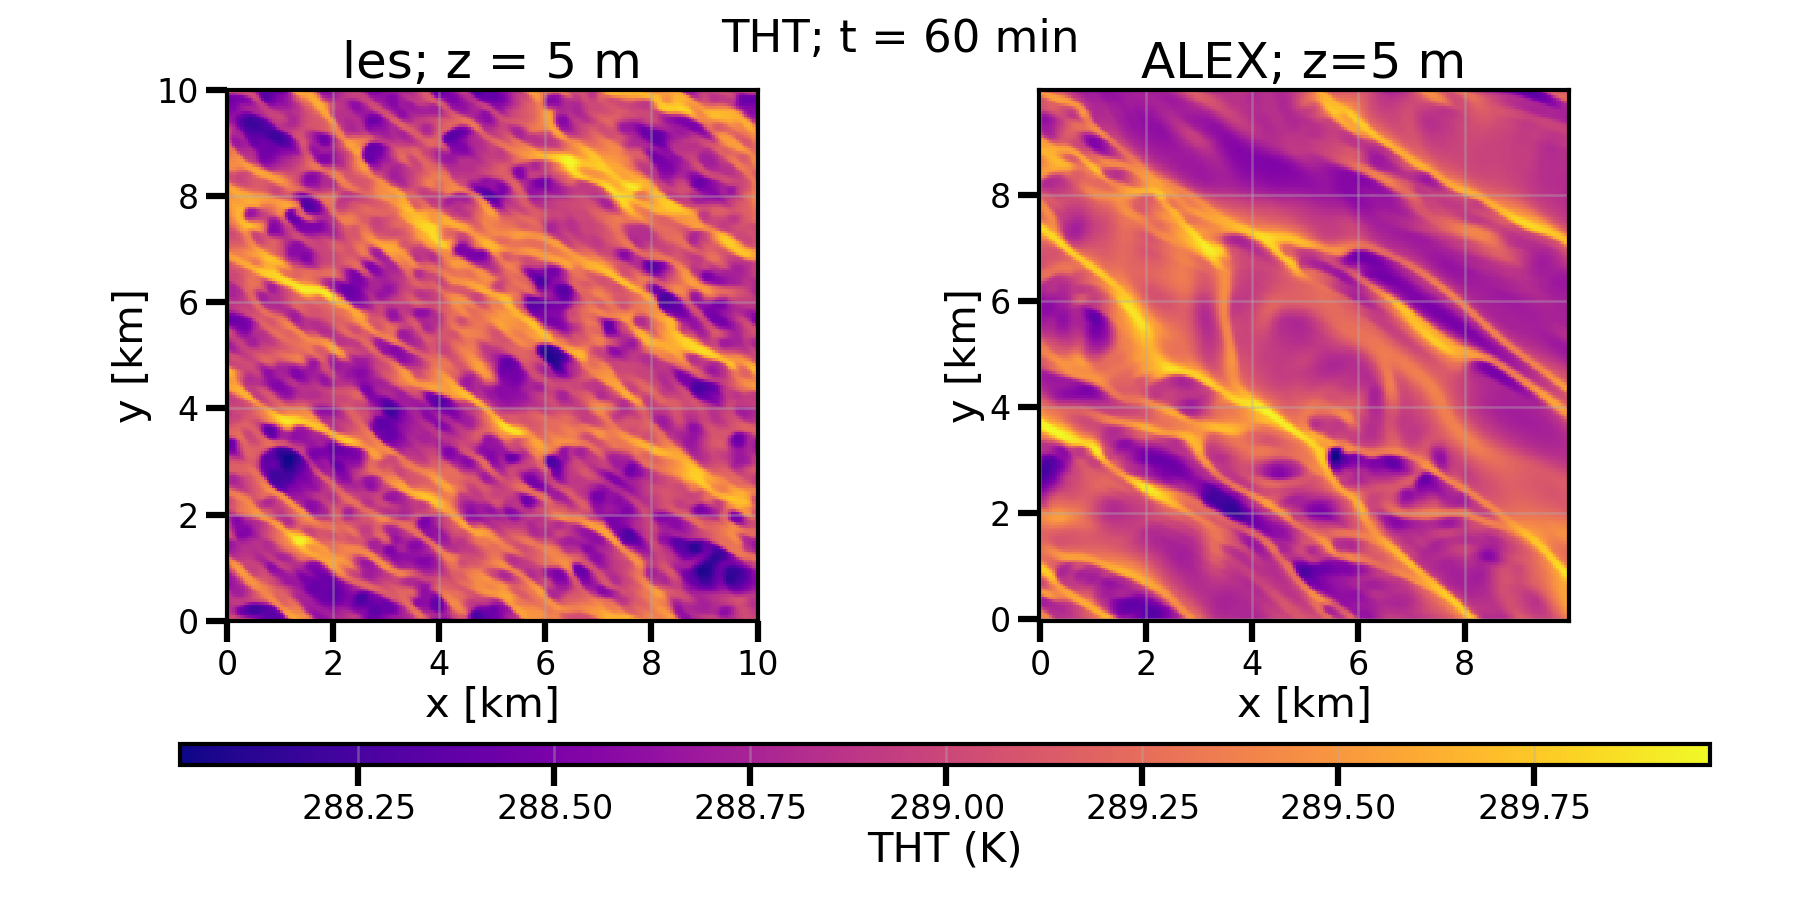
\includegraphics[width=1\linewidth]{diff/compTHT.png}
	\end{minipage}
	\hfill
	\begin{minipage}{0.48\textwidth}
		REAL - LES \\
		\centering
		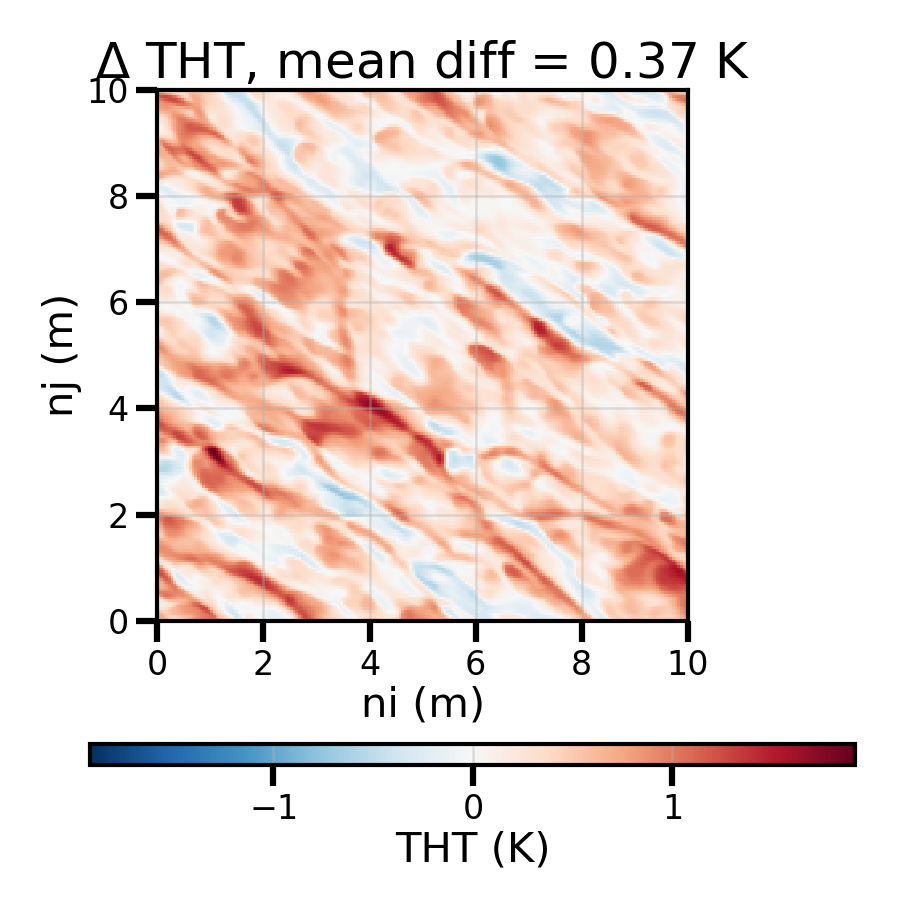
\includegraphics[width=0.7\linewidth]{diff/diffTHT.png}
		\vspace{0.5cm}
	\end{minipage}
$theta_r > \theta_i \implies \Delta \theta_r > \Delta \theta_i \implies H_r > H_i $
\end{frame}


\subsection{Piste4: Différence de sst!}
\begin{frame}{Différence de sst}
	Je n'avais pas la même sst: car sst varie dans le domaine dans ALEX
	\begin{minipage}{0.48\textwidth}
		\centering
		\begin{tabular}{|c|cc|}
			\hline
			LES &  SST  & 289.94  $\rightarrow $ 292.90 K \\
				&  $\Theta$ & 288.55 K $\rightarrow$ 288.67 K\\
				& $\Delta \Theta $ &  1.39  $\rightarrow$ 4.23K \\	
			\hline
			REAL &  SST  & 292.90 K \\
			 		&  $\Theta$ & 289.39 K\\
				& $\Delta \Theta $ &  3.52 K \\	
			\hline
		\end{tabular} \\
				\vspace{0.5cm}
	Grosse erreur dans les flux latents car pas de nudging de l'humidité ?
	\end{minipage}
	\hfill
	\begin{minipage}{0.48\textwidth}
		\centering
		
\includegraphics[width=1\linewidth]{newSST/comp_cut.png}
		\begin{tabular}{c|cc}
			&  LHF   & SHF \\
			\hline
			LES  & \hl{667.32} &  212.56  \\
			ALEX & 451.15 & 280.33 \\
		\end{tabular} \\
		\vspace{0.5cm}
	\end{minipage}
\end{frame}

\begin{frame}{Avec rv nudgé}

\begin{minipage}{0.48\textwidth}
		\centering
\begin{figure}
	\centering
	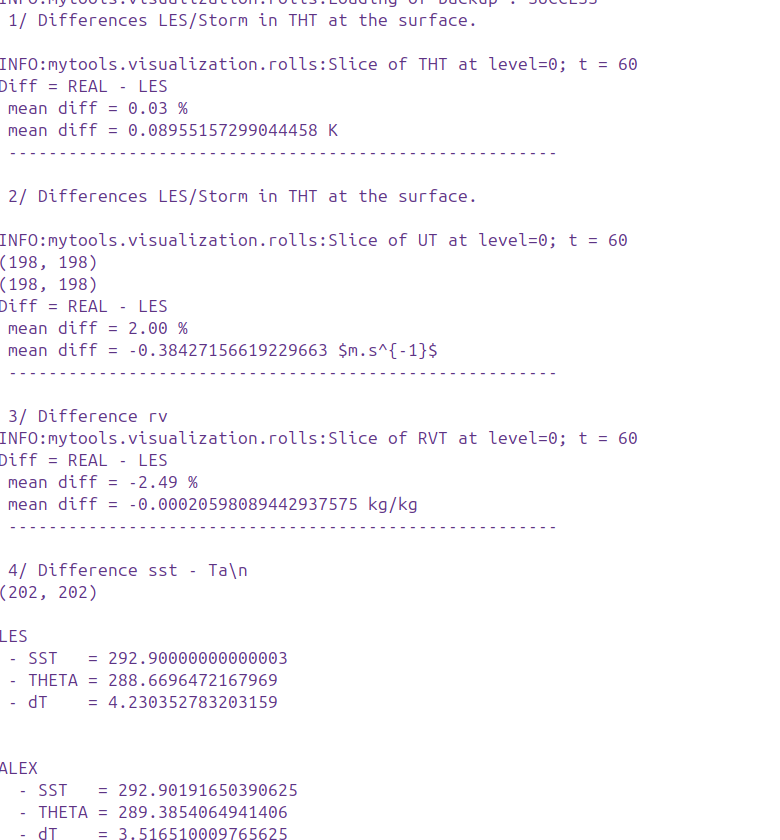
\includegraphics[width=0.5\linewidth]{FIGURES/newSST/shf_flux}
\end{figure}
$\implies$ les champs nudgé ont une moyenne proche du REAL case, explication ??
	\end{minipage}
	\hfill
	\begin{minipage}{0.48\textwidth}
		\centering
		
\includegraphics[width=1\linewidth]{newSST/comp_cut.png}
		\begin{tabular}{c|cc}
			&  LHF   & SHF \\
			\hline
			LES  & \hl{667.32} &  212.56  \\
			ALEX & 451.15 & 280.33 \\
		\end{tabular} \\
		\vspace{0.5cm}
	\end{minipage}
\end{frame}

\begin{frame}{Avec rv nudgé}
	
	\begin{minipage}{0.48\textwidth}
		\centering
		\begin{figure}
			\centering
			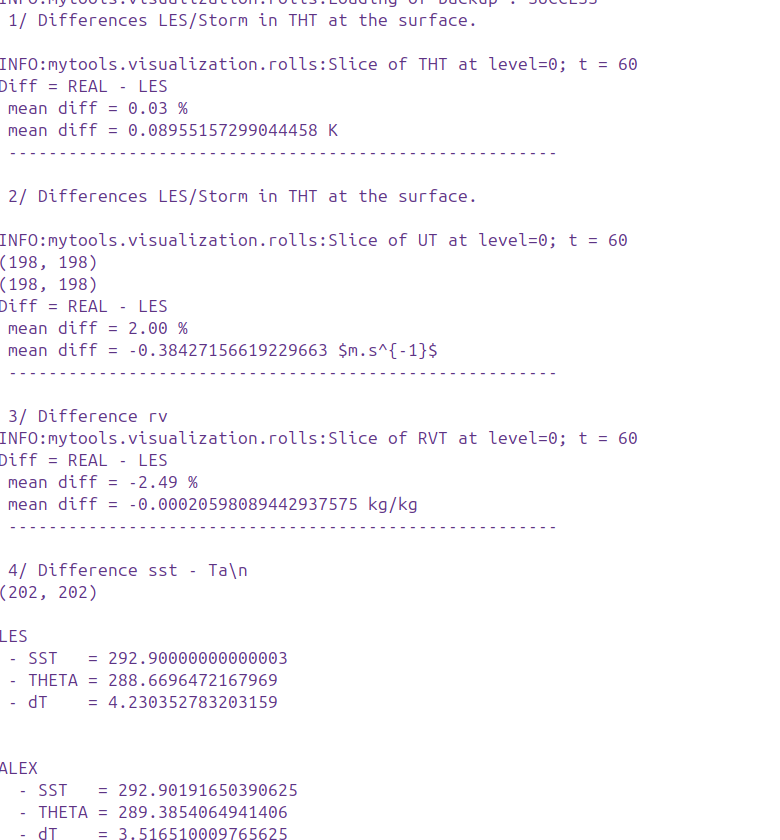
\includegraphics[width=0.5\linewidth]{FIGURES/newSST/shf_flux}
		\end{figure}
		$\implies$ les champs nudgé ont une moyenne proche du REAL case, explication ??
	\end{minipage}
	\hfill
	\begin{minipage}{0.48\textwidth}
		\centering
		
\includegraphics[width=1\linewidth]{newSST/comp_cut.png}
		\begin{tabular}{c|cc}
			&  LHF   & SHF \\
			\hline
			LES  & \hl{667.32} &  212.56  \\
			ALEX & 451.15 & 280.33 \\
		\end{tabular} \\
		\vspace{0.5cm}
	\end{minipage}
\end{frame}


\begin{frame}	
	On peut s'interroger sur la sst: sst moyenné a-t-elle un impact ? \\
	On pourrait sy attendre car LE depend de $\Delta q$ et $q{sat}$ depend de la température de la mer. 
	\begin{minipage}{\textwidth}
		\centering
		\begin{figure}
			\centering
			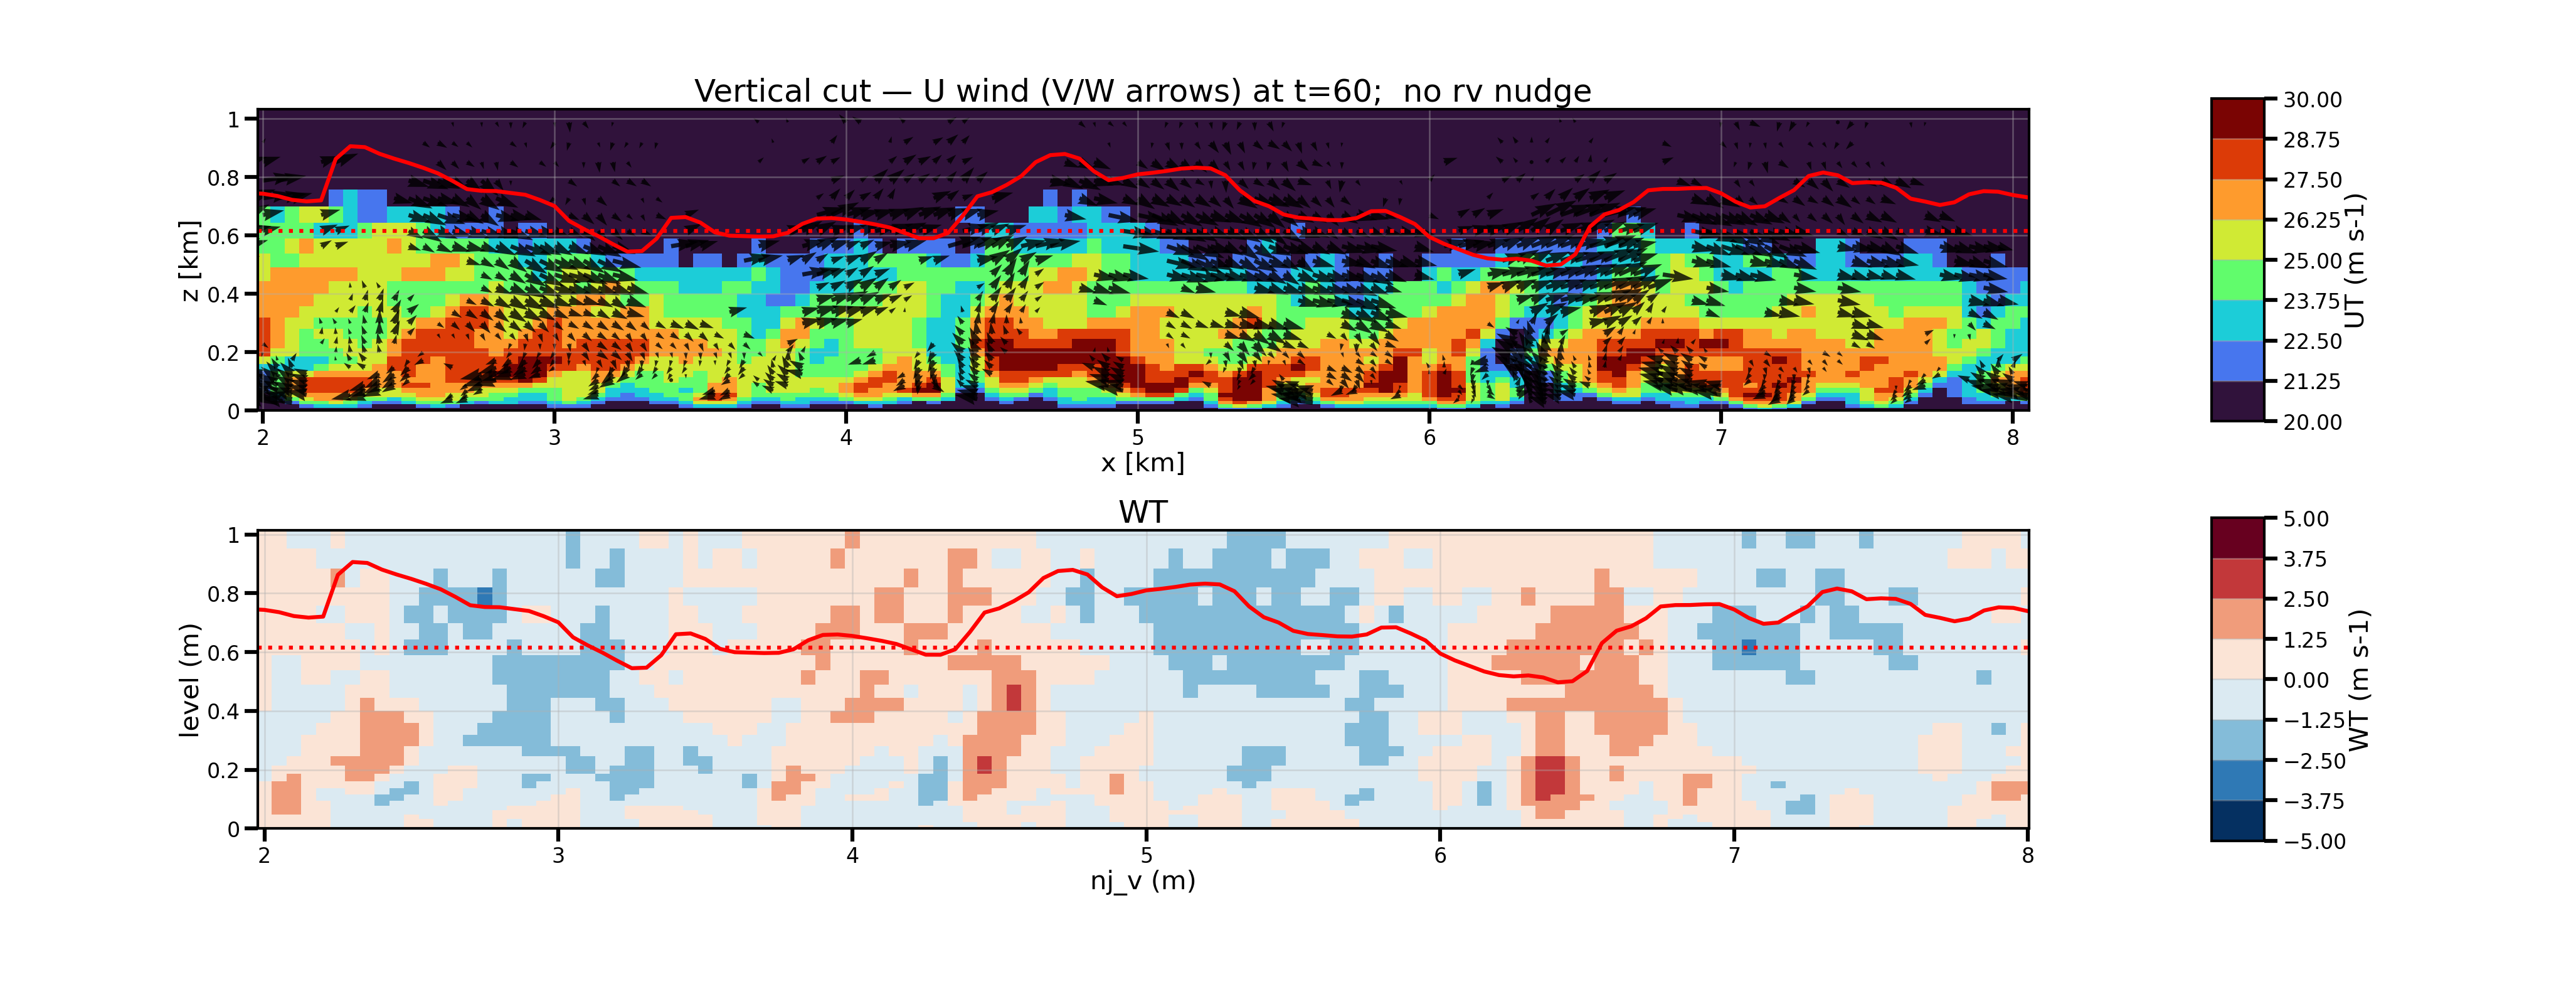
\includegraphics[width=\linewidth]{FIGURES/newSST/beautiful_cut}
			\caption{Vertical cut of the wind components}
			\label{fig:shfflux}
		\end{figure}
	\end{minipage}
\end{frame}


\begin{frame}{Fonction d'auto-corrélation R}
	\begin{minipage}{0.48\textwidth}
		Les structures sont similaire entre REAL and IDEAL cases. \\ 
		\centering
		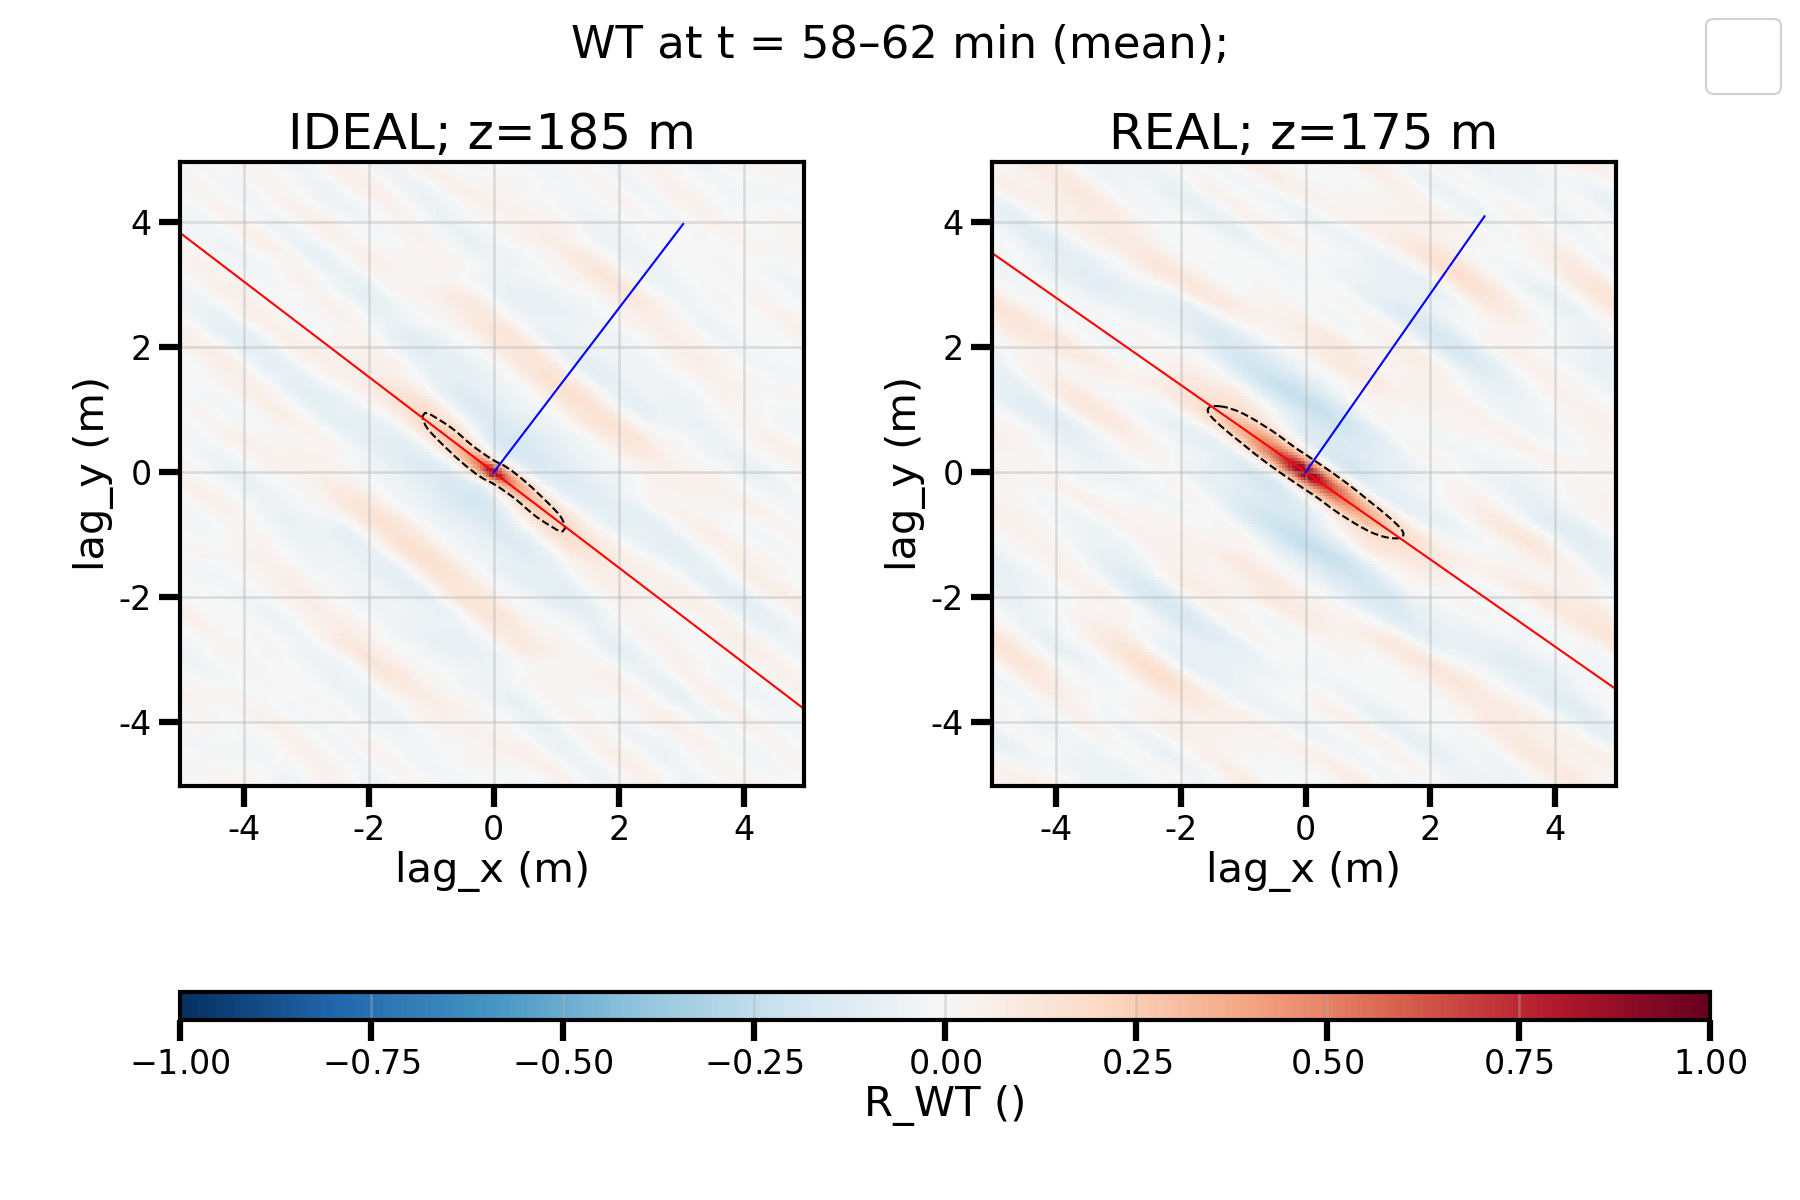
\includegraphics[width=1\linewidth]{newSST/acf.png}
	\end{minipage}
	\hfill
	\begin{minipage}{0.48\textwidth}
		\centering
		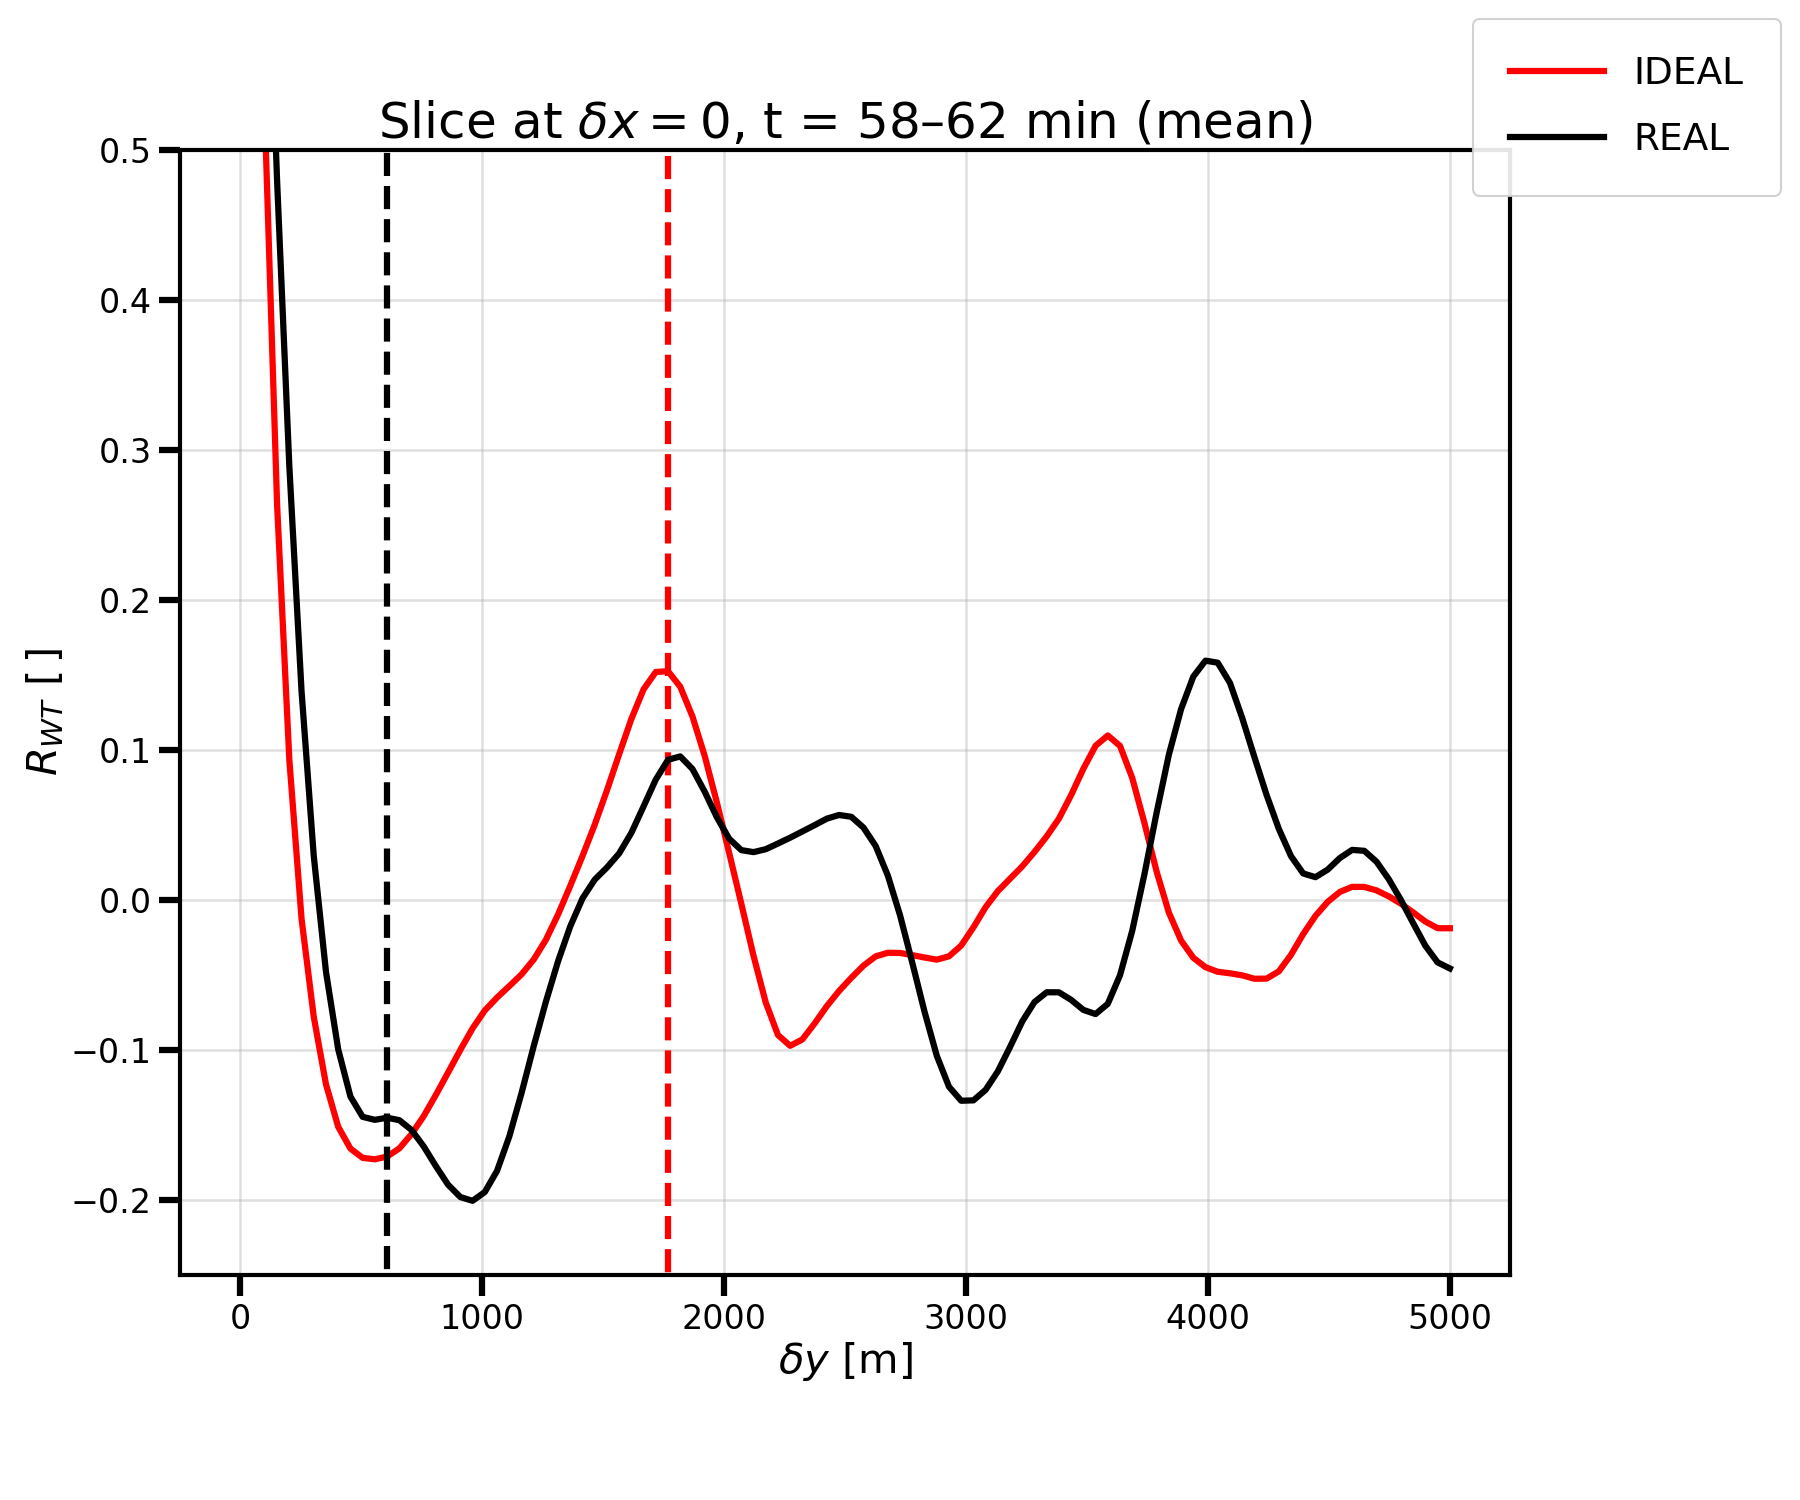
\includegraphics[width=1\linewidth]{newSST/acf_slice.png}
		\vspace{0.5cm}
	\end{minipage}
\end{frame}


% =======================================================================================
% =======================================================================================
\section{Large scale à LES}
\begin{frame}
	\sectionpage
\end{frame}
\begin{frame}{Large Scale to LES?}
	\textbf{Objectif}: D'un profil grande échelle, obtenir une simulation LES ? \\
	Départ de la simulation à 800m de Nicolas.  \\
	\begin{minipage}{0.35\textwidth}
		\centering
		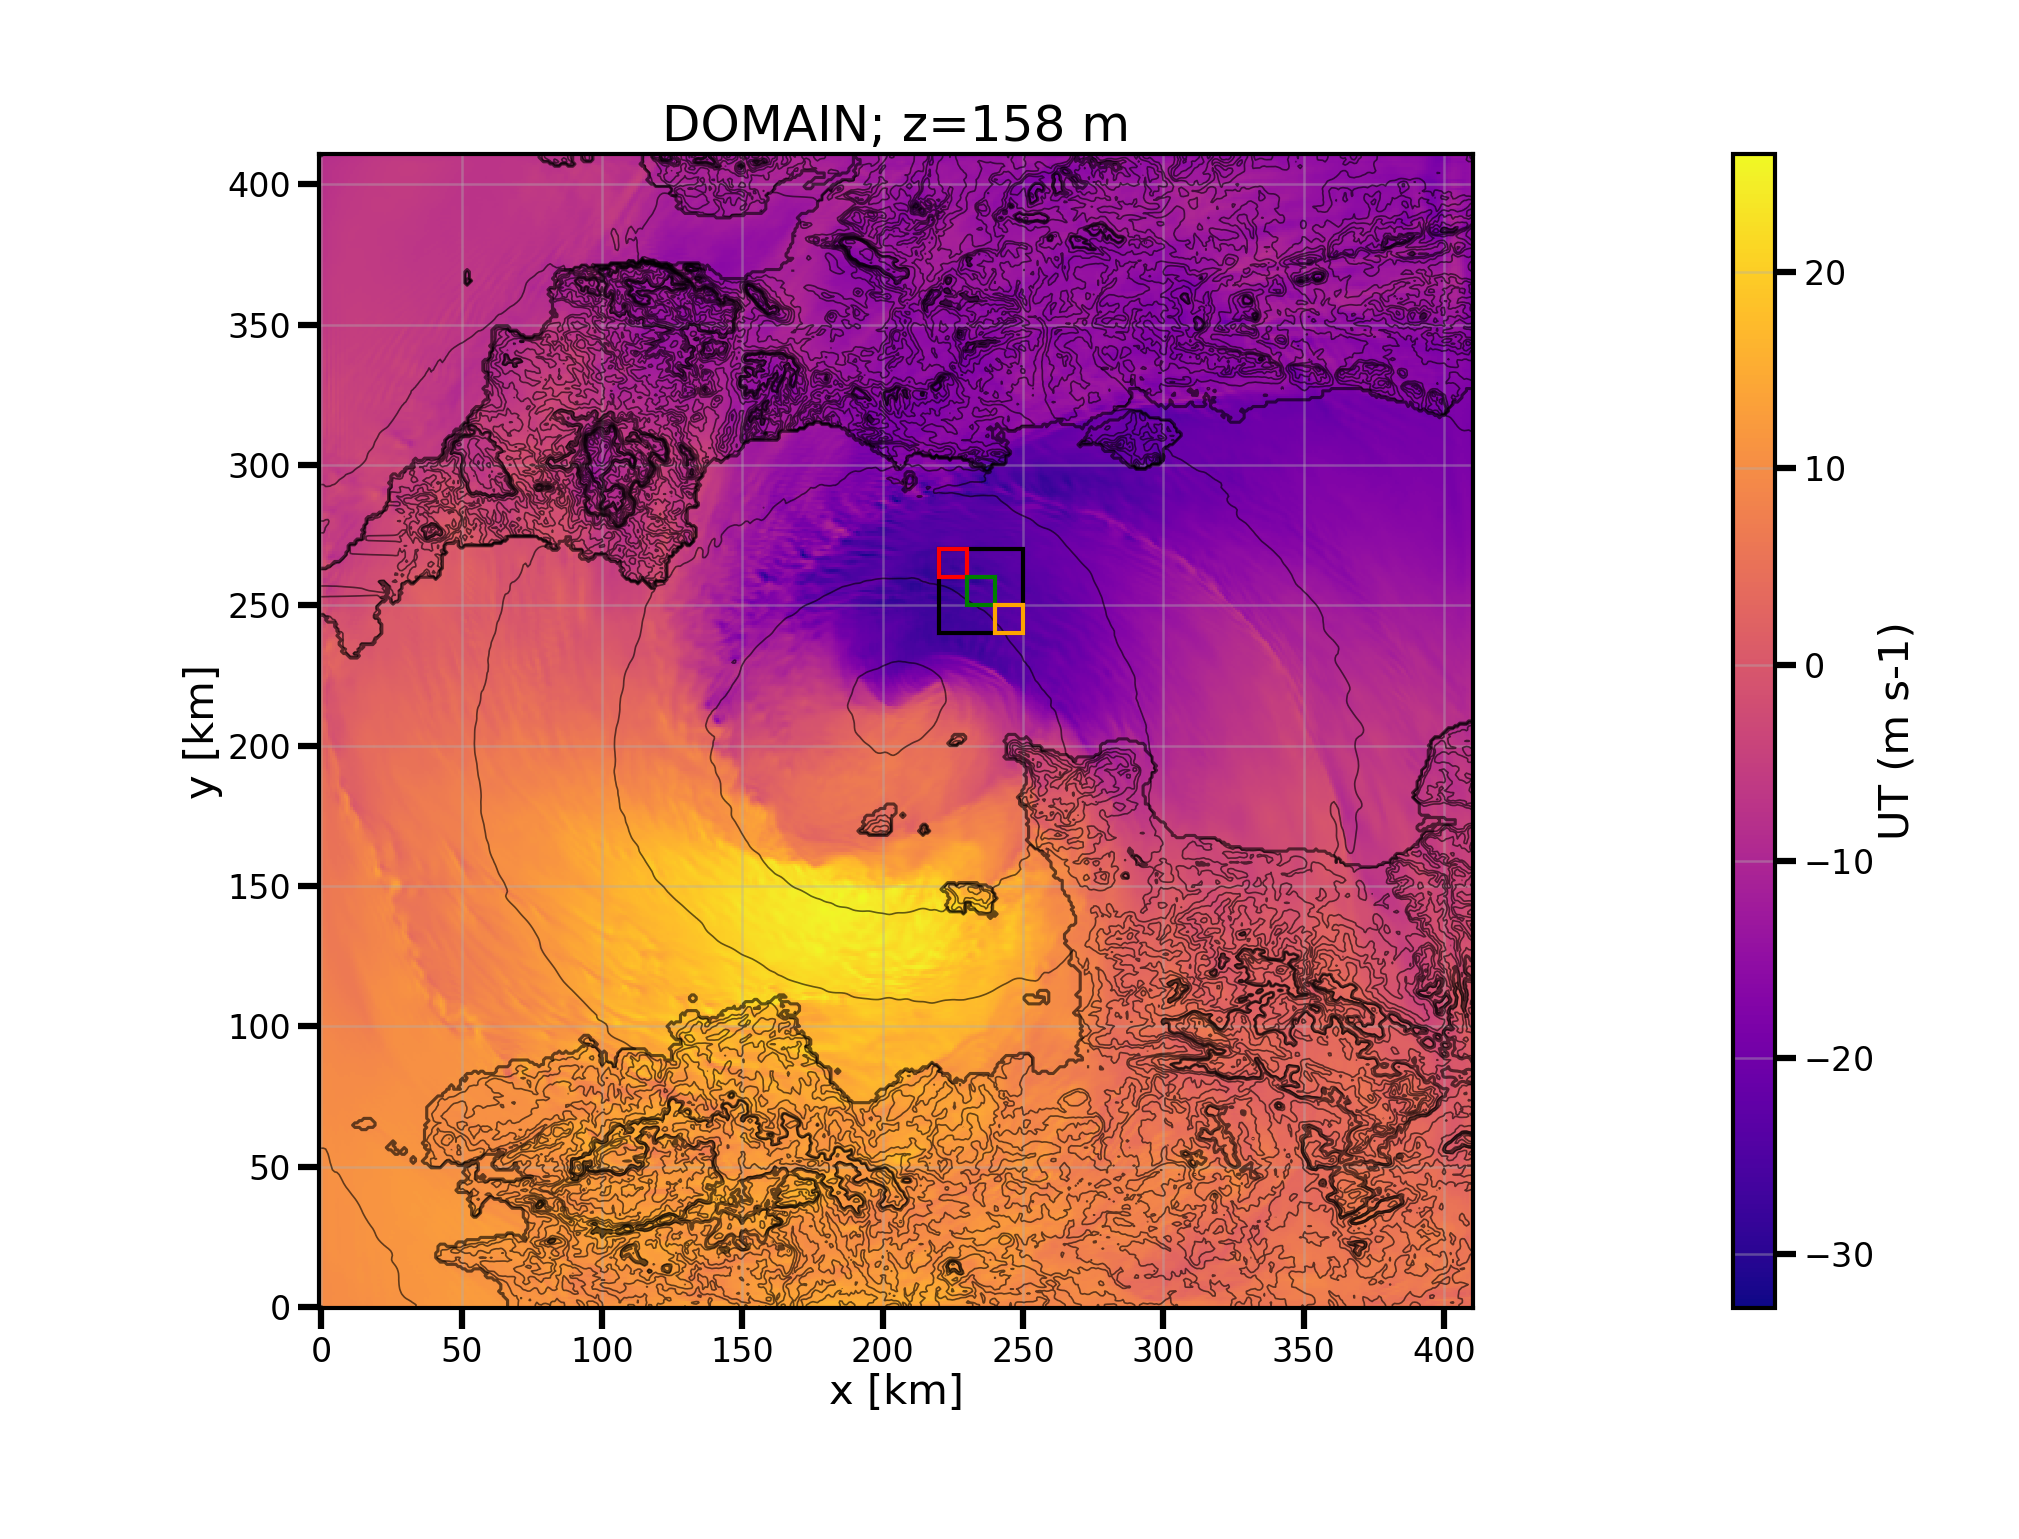
\includegraphics[width=\linewidth]{bigDOM/bigDOM.png}
	\end{minipage}
	\hfill
	\begin{minipage}{0.55\textwidth}
		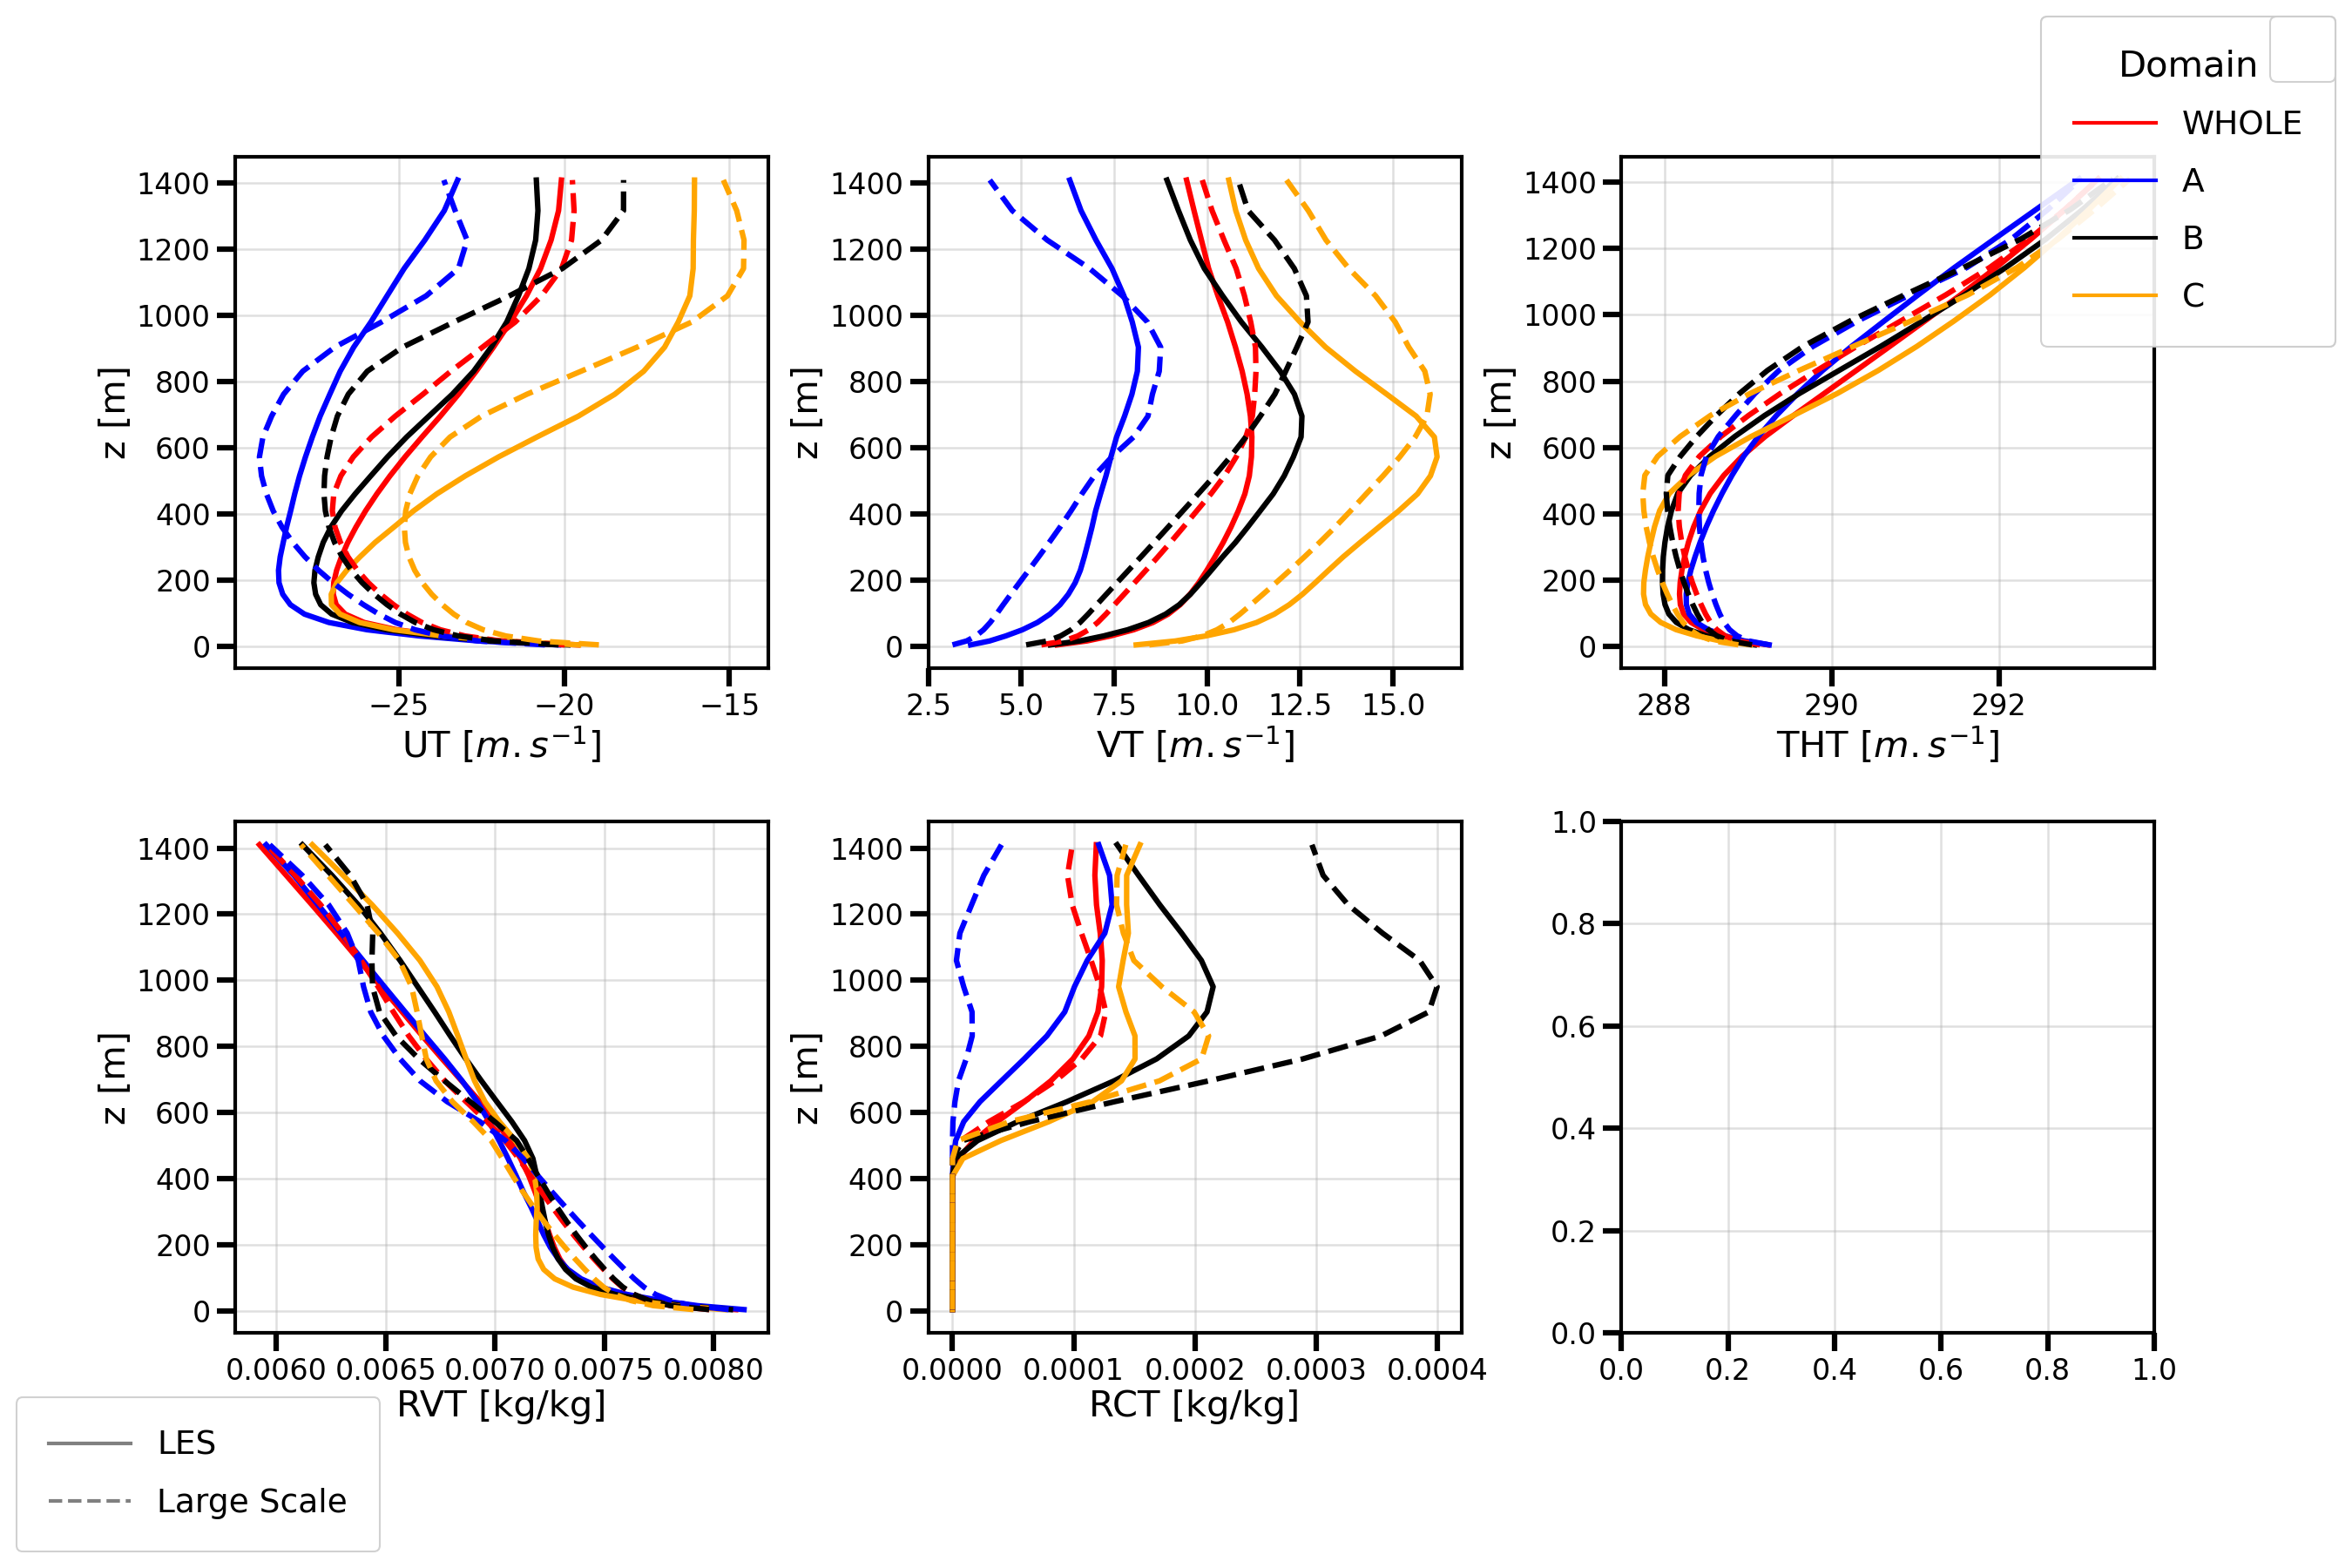
\includegraphics[width=\linewidth]{bigDOM/profile.png}
	\end{minipage} \\
	Limitation est le nudging: impose une position à ce jet et empêche le transfert du vent moyen vers les couches les plus  basses.  \\
\end{frame}

\begin{frame}{Idée : Nudging adaptatif ?}
	Implémentation d'un nudging qui suit les variations du profil vertical et notamment de la descente du jet vers les basses couches. \\
	\vfill
	$$ \partial_t \phi = - \frac{\alpha(z,t)}{\tau} \left( \langle \phi \rangle (z) - \phi_{LS}(z) \right) $$
	où $\alpha(z,t)$ est fixe et égal à 1 maintenant. \\
	Mais pourrait dépendre de la position du jet $z_{jet}$ ? \\
	Propositions: centre de cisaillement, max ??
	$$ z_{jet} = \frac{\int \left(\partial_z\langle U \rangle \right) ^2 z dz }{\int \left(\partial_z\langle U \rangle \right)^2 dz } $$ \\
	$$ z_{jet} = max \left( \langle U \rangle (z) \right) $$
	\vfill
	Problème: possibilité de force de nudging qui "saute" : lissage/amortissement sur le temps. 
\end{frame}
\end{document}   
